

\input{../Latex_Templates/Preamble_Report}

%%%%% TITLE PAGE

%\subject{, VT23}
\title{ Report for the Course Modelling in Computational Science, HT23 \\[1ex]
	  \large Project 2: Cell reprogramming}
%\subtitle{}
\author{Theo Koppenhöfer \\[1ex] (with Jimmy Gunnarson)}
\date{Lund \\[1ex] \today}

\addbibresource{bibliography.bib}

\usepackage{pythonhighlight}
\usepackage{pgfplots}
\graphicspath{{../Plots/}}

\pgfplotsset{
	compat=newest,
    every axis/.append style={
        axis y line=left,
        axis x line=bottom,
        scale only axis,
%    	max space between ticks=25pt,
        width=0.7\textwidth,
        scaled ticks=true,
        axis line style={thick,-,>=latex, shorten >=-.4cm},
    		x tick label style={
		    /pgf/number format/precision=3
		}
    },
    every axis plot/.append style={thick},
    tick style={black, thick}
}

%%%%% The content starts here %%%%%%%%%%%%%


\begin{document}

\maketitle

\section{Introduction}

\section{The setup}

\section{The experiments}

\begin{figure}
\centering
\begin{minipage}{0.7\textwidth}
\centering
\graphicspath{{../Plots/}}
% This file was created with tikzplotlib v0.10.1.
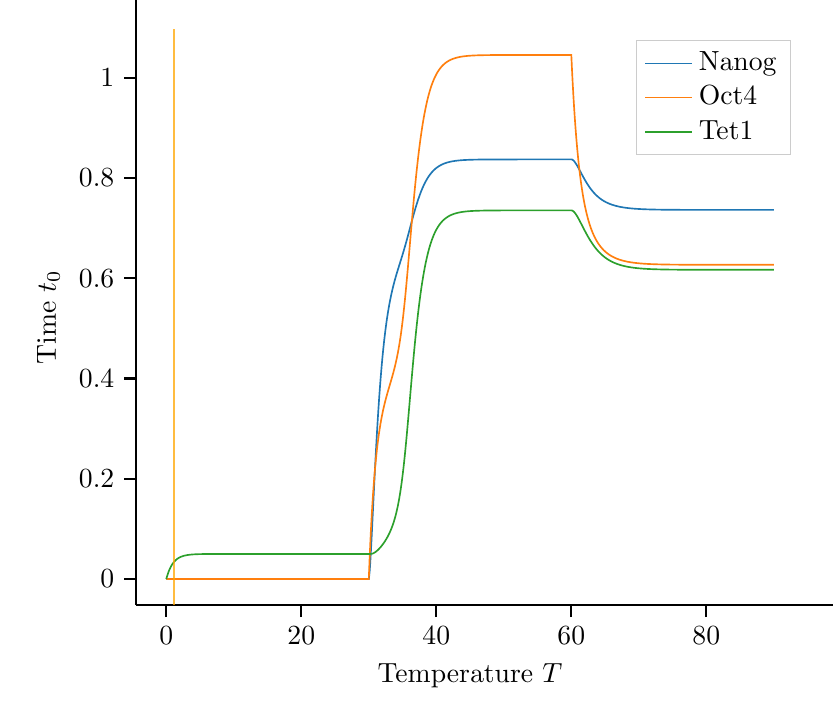
\begin{tikzpicture}

\definecolor{darkgray176}{RGB}{176,176,176}
\definecolor{darkorange25512714}{RGB}{255,127,14}
\definecolor{forestgreen4416044}{RGB}{44,160,44}
\definecolor{lightgray204}{RGB}{204,204,204}
\definecolor{orange}{RGB}{255,165,0}
\definecolor{steelblue31119180}{RGB}{31,119,180}

\begin{axis}[
legend cell align={left},
legend style={fill opacity=0.8, draw opacity=1, text opacity=1, draw=lightgray204},
tick align=outside,
tick pos=left,
x grid style={darkgray176},
xlabel={Temperature \(\displaystyle T\)},
xmin=-4.5, xmax=94.5,
xtick style={color=black},
y grid style={darkgray176},
ylabel={Time \(\displaystyle t_0\)},
ymin=-0.052267093893759, ymax=1.09760897176894,
ytick style={color=black}
]
\addplot [semithick, steelblue31119180]
table {%
0 0
0.0001 0
0.0011 0
0.0111 0
0.1111 0
0.2111 0
0.3111 0
0.4111 0
0.5111 0
0.6111 0
0.7111 0
0.8111 0
0.9111 0
1.0111 0
1.1111 0
1.2111 0
1.3111 0
1.4111 0
1.5111 0
1.6111 0
1.7111 0
1.8111 0
1.9111 0
2.0111 0
2.1111 0
2.2111 0
2.3111 0
2.4111 0
2.5111 0
2.6111 0
2.7111 0
2.8111 0
2.9111 0
3.0111 0
3.1111 0
3.2111 0
3.3111 0
3.4111 0
3.5111 0
3.6111 0
3.7111 0
3.8111 0
3.9111 0
4.0111 0
4.1111 0
4.2111 0
4.3111 0
4.4111 0
4.5111 0
4.6111 0
4.7111 0
4.8111 0
4.9111 0
5.0111 0
5.1111 0
5.2111 0
5.3111 0
5.4111 0
5.5111 0
5.6111 0
5.7111 0
5.8111 0
5.9111 0
6.0111 0
6.1111 0
6.21109999999999 0
6.31109999999999 0
6.41109999999999 0
6.51109999999999 0
6.61109999999999 0
6.71109999999999 0
6.81109999999999 0
6.91109999999999 0
7.01109999999999 0
7.11109999999999 0
7.21109999999999 0
7.31109999999999 0
7.41109999999999 0
7.51109999999999 0
7.61109999999999 0
7.71109999999999 0
7.81109999999999 0
7.91109999999999 0
8.01109999999999 0
8.11109999999999 0
8.21109999999999 0
8.31109999999999 0
8.41109999999999 0
8.51109999999999 0
8.61109999999999 0
8.71109999999999 0
8.81109999999999 0
8.91109999999999 0
9.01109999999998 0
9.11109999999998 0
9.21109999999998 0
9.31109999999998 0
9.41109999999998 0
9.51109999999998 0
9.61109999999998 0
9.71109999999998 0
9.81109999999998 0
9.91109999999998 0
10.0111 0
10.1111 0
10.2111 0
10.3111 0
10.4111 0
10.5111 0
10.6111 0
10.7111 0
10.8111 0
10.9111 0
11.0111 0
11.1111 0
11.2111 0
11.3111 0
11.4111 0
11.5111 0
11.6111 0
11.7111 0
11.8111 0
11.9111 0
12.0111 0
12.1111 0
12.2111 0
12.3111 0
12.4111 0
12.5111 0
12.6111 0
12.7111 0
12.8111 0
12.9111 0
13.0111 0
13.1111 0
13.2111 0
13.3111 0
13.4111 0
13.5111 0
13.6111 0
13.7111 0
13.8111 0
13.9111 0
14.0111 0
14.1111 0
14.2111 0
14.3111 0
14.4111 0
14.5111 0
14.6111 0
14.7111 0
14.8111 0
14.9111 0
15.0111 0
15.1111 0
15.2111 0
15.3111 0
15.4111 0
15.5111 0
15.6111 0
15.7111 0
15.8111 0
15.9111 0
16.0111 0
16.1111 0
16.2111 0
16.3111 0
16.4111 0
16.5111 0
16.6111 0
16.7111 0
16.8111 0
16.9111 0
17.0111 0
17.1111 0
17.2111 0
17.3111 0
17.4111 0
17.5111 0
17.6111 0
17.7111 0
17.8111 0
17.9111 0
18.0111 0
18.1111 0
18.2111 0
18.3111 0
18.4111 0
18.5111 0
18.6111 0
18.7111 0
18.8111 0
18.9111 0
19.0111 0
19.1111 0
19.2111 0
19.3111 0
19.4111 0
19.5111 0
19.6111 0
19.7111 0
19.8111 0
19.9111 0
20.0111 0
20.1111 0
20.2111 0
20.3111 0
20.4111 0
20.5111 0
20.6111 0
20.7111 0
20.8111 0
20.9111 0
21.0111 0
21.1111 0
21.2111 0
21.3111 0
21.4111 0
21.5111 0
21.6111 0
21.7111 0
21.8111 0
21.9111 0
22.0111 0
22.1111 0
22.2111 0
22.3111 0
22.4111000000001 0
22.5111000000001 0
22.6111000000001 0
22.7111000000001 0
22.8111000000001 0
22.9111000000001 0
23.0111000000001 0
23.1111000000001 0
23.2111000000001 0
23.3111000000001 0
23.4111000000001 0
23.5111000000001 0
23.6111000000001 0
23.7111000000001 0
23.8111000000001 0
23.9111000000001 0
24.0111000000001 0
24.1111000000001 0
24.2111000000001 0
24.3111000000001 0
24.4111000000001 0
24.5111000000001 0
24.6111000000001 0
24.7111000000001 0
24.8111000000001 0
24.9111000000001 0
25.0111000000001 0
25.1111000000001 0
25.2111000000001 0
25.3111000000001 0
25.4111000000001 0
25.5111000000001 0
25.6111000000001 0
25.7111000000001 0
25.8111000000001 0
25.9111000000001 0
26.0111000000001 0
26.1111000000001 0
26.2111000000001 0
26.3111000000001 0
26.4111000000001 0
26.5111000000001 0
26.6111000000001 0
26.7111000000001 0
26.8111000000001 0
26.9111000000001 0
27.0111000000001 0
27.1111000000001 0
27.2111000000001 0
27.3111000000001 0
27.4111000000001 0
27.5111000000001 0
27.6111000000001 0
27.7111000000001 0
27.8111000000001 0
27.9111000000001 0
28.0111000000001 0
28.1111000000001 0
28.2111000000001 0
28.3111000000001 0
28.4111000000001 0
28.5111000000001 0
28.6111000000001 0
28.7111000000001 0
28.8111000000001 0
28.9111000000001 0
29.0111000000001 0
29.1111000000001 0
29.2111000000001 0
29.3111000000001 0
29.4111000000002 0
29.5111000000002 0
29.6111000000002 0
29.7111000000002 0
29.8111000000002 0
29.9111000000002 0
30 0
30 0
30.0026862579625 0.000165271778314076
30.0295488375876 0.00224894953969477
30.1295488375876 0.0157049231076706
30.2295488375876 0.0355802208094795
30.3295488375876 0.0594516102440574
30.4295488375876 0.0856881376128742
30.5295488375876 0.113166666378529
30.6295488375876 0.141102086589483
30.7295488375876 0.168941576776403
30.8295488375876 0.196296245646282
30.9295488375876 0.222895341093683
31.0295488375876 0.248554581397234
31.1295488375876 0.273153656362102
31.2295488375876 0.29661989187759
31.3295488375876 0.318916183631431
31.4295488375876 0.340031963626061
31.5295488375876 0.359976366799672
31.6295488375876 0.378773021553809
31.7295488375876 0.396456056210401
31.8295488375876 0.413067026842002
31.9295488375876 0.428652550246605
32.0295488375876 0.443262481064565
32.1295488375876 0.456948511681013
32.2295488375876 0.469763102469694
32.3295488375876 0.48175867131239
32.4295488375876 0.49298698732897
32.5295488375876 0.503498725858178
32.6295488375876 0.513343150973326
32.7295488375876 0.522567898933376
32.8295488375876 0.531218841484601
32.9295488375876 0.539340012222673
33.0295488375876 0.546973582578406
33.1295488375876 0.554159876607141
33.2295488375876 0.560937415792086
33.3295488375876 0.567342986625263
33.4295488375876 0.573411724884714
33.5295488375876 0.579177211338099
33.6295488375876 0.584671574107782
33.7295488375876 0.589925593155452
33.8295488375876 0.594968802302665
33.9295488375876 0.599829583915682
34.0295488375876 0.604535250877082
34.1295488375876 0.609112109795462
34.2295488375876 0.613585498662289
34.3295488375876 0.617979791507637
34.4295488375876 0.622318362271002
34.5295488375876 0.626623500417171
34.6295488375876 0.630916272193819
34.7295488375876 0.635216324271956
34.8295488375876 0.639541631164998
34.9295488375876 0.643908194355722
35.0295488375876 0.648329709076524
35.1295488375876 0.652817223173581
35.2295488375876 0.657378819813231
35.3295488375876 0.662019359986174
35.4295488375876 0.666740320050627
35.5295488375876 0.671539753011703
35.6295488375876 0.676412390330154
35.7295488375876 0.681349885727564
35.8295488375876 0.686341186637107
35.9295488375876 0.691373005684032
36.0295488375876 0.696430356126911
36.1295488375876 0.701497112469163
36.2295488375876 0.706556560008584
36.3295488375876 0.711591903504319
36.4295488375876 0.716586713588238
36.5295488375876 0.72152529834118
36.6295488375876 0.726392995348253
36.7295488375877 0.731176385835001
36.8295488375877 0.735863436936678
36.9295488375877 0.740443580870694
37.0295488375877 0.744907741059055
37.1295488375877 0.749248315442228
37.2295488375877 0.753459126685758
37.3295488375877 0.757535348000218
37.4295488375877 0.761473412099721
37.5295488375877 0.765270909574292
37.6295488375877 0.768926481750606
37.7295488375877 0.772439712024345
37.8295488375877 0.775811018694726
37.9295488375877 0.779041551525711
38.0295488375877 0.782133093593854
38.1295488375877 0.78508796944736
38.2295488375877 0.787908960178673
38.3295488375877 0.790599225687161
38.4295488375877 0.793162234162847
38.5295488375877 0.795601698642038
38.6295488375877 0.797921520358127
38.7295488375877 0.800125738524684
38.8295488375877 0.802218486134142
38.9295488375877 0.804203951326125
39.0295488375877 0.806086343868836
39.1295488375877 0.807869866299839
39.2295488375877 0.809558689285265
39.3295488375877 0.811156930775889
39.4295488375877 0.812668638562278
39.5295488375877 0.814097775857597
39.6295488375877 0.815448209564295
39.7295488375877 0.816723700908761
39.8295488375877 0.817927898155529
39.9295488375877 0.819064331139056
40.0295488375877 0.820136407376364
40.1295488375877 0.82114740954752
40.2295488375877 0.822100494153043
40.3295488375877 0.822998691177777
40.4295488375877 0.82384490460955
40.5295488375877 0.824641913678097
40.6295488375877 0.825392374695367
40.7295488375877 0.826098823392457
40.8295488375877 0.826763677661187
40.9295488375877 0.827389240619817
41.0295488375877 0.827977703932701
41.1295488375877 0.828531151322876
41.2295488375877 0.82905156222479
41.3295488375877 0.829540815531692
41.4295488375877 0.830000693398668
41.5295488375877 0.830432885068059
41.6295488375877 0.830838990689057
41.7295488375877 0.831220525107744
41.8295488375877 0.831578921607753
41.9295488375877 0.831915535585185
42.0295488375877 0.832231648144427
42.1295488375877 0.832528469604102
42.2295488375877 0.832807142904725
42.3295488375877 0.833068746911556
42.4295488375877 0.833314299607899
42.5295488375877 0.833544761175514
42.6295488375877 0.833761036960118
42.7295488375877 0.83396398032098
42.8295488375877 0.834154395364556
42.9295488375877 0.834333039562854
43.0295488375877 0.834500626257858
43.1295488375877 0.834657827053894
43.2295488375877 0.834805274100209
43.3295488375877 0.834943562266434
43.4295488375877 0.835073251213827
43.5295488375877 0.835194867365456
43.6295488375877 0.83530890577858
43.7295488375877 0.835415831922674
43.8295488375878 0.835516083366534
43.9295488375878 0.835610071377999
44.0295488375878 0.835698182439808
44.1295488375878 0.835780779685093
44.2295488375878 0.835858204255984
44.3295488375878 0.835930776588736
44.4295488375878 0.835998797628744
44.5295488375878 0.836062549978701
44.6295488375878 0.836122298983097
44.7295488375878 0.836178293752149
44.8295488375878 0.836230768128153
44.9295488375878 0.83627994159715
45.0295488375878 0.8363260201487
45.1295488375878 0.836369197086424
45.2295488375878 0.836409653791905
45.3295488375878 0.836447560444413
45.4295488375878 0.836483076698796
45.5295488375878 0.836516352323817
45.6295488375878 0.836547527803071
45.7295488375878 0.836576734900549
45.8295488375878 0.836604097192794
45.9295488375878 0.836629730569531
46.0295488375878 0.836653743704507
46.1295488375878 0.836676238498261
46.2295488375878 0.836697310494389
46.3295488375878 0.836717049270844
46.4295488375878 0.836735538807679
46.5295488375878 0.836752857832619
46.6295488375878 0.836769080145735
46.7295488375878 0.836784274924435
46.8295488375878 0.836798507009933
46.9295488375878 0.836811837176284
47.0295488375878 0.836824322383004
47.1295488375878 0.836836016012261
47.2295488375878 0.836846968091536
47.3295488375878 0.83685722550264
47.4295488375878 0.836866832177883
47.5295488375878 0.836875829284184
47.6295488375878 0.836884255395828
47.7295488375878 0.836892146656569
47.8295488375878 0.836899536931719
47.9295488375878 0.836906457950822
48.0295488375878 0.836912939441492
48.1295488375878 0.836919009254959
48.2295488375878 0.836924693483805
48.3295488375878 0.836930016572394
48.4295488375878 0.836935001420429
48.5295488375878 0.836939669480055
48.6295488375878 0.83694404084691
48.7295488375878 0.836948134345497
48.8295488375878 0.836951967609225
48.9295488375878 0.83695555715544
49.0295488375878 0.836958918455771
49.1295488375878 0.836962066002065
49.2295488375878 0.836965013368199
49.3295488375878 0.836967773268009
49.4295488375878 0.836970357609589
49.5295488375878 0.836972777546181
49.6295488375878 0.83697504352387
49.7295488375878 0.836977165326274
49.8295488375878 0.836979152116435
49.9295488375878 0.836981012476065
50.0295488375878 0.836982754442324
50.1295488375878 0.836984385542284
50.2295488375878 0.836985912825217
50.3295488375878 0.836987342892853
50.4295488375878 0.83698868192772
50.5295488375878 0.836989935719709
50.6295488375878 0.83699110969095
50.7295488375878 0.836992208919126
50.8295488375879 0.836993238159306
50.9295488375879 0.836994201864406
51.0295488375879 0.836995104204353
51.1295488375879 0.836995949084034
51.2295488375879 0.836996740160116
51.3295488375879 0.836997480856798
51.4295488375879 0.836998174380565
51.5295488375879 0.83699882373401
51.6295488375879 0.836999431728781
51.7295488375879 0.837000000997705
51.8295488375879 0.837000534006146
51.9295488375879 0.837001033062644
52.0295488375879 0.837001500328878
52.1295488375879 0.837001937828995
52.2295488375879 0.837002347458353
52.3295488375879 0.837002730991705
52.4295488375879 0.837003090090865
52.5295488375879 0.83700342631189
52.6295488375879 0.837003741111798
52.7295488375879 0.837004035854872
52.8295488375879 0.837004311818554
52.9295488375879 0.837004570198967
53.0295488375879 0.837004812116088
53.1295488375879 0.837005038618594
53.2295488375879 0.837005250688393
53.3295488375879 0.837005449244876
53.4295488375879 0.837005635148891
53.5295488375879 0.837005809206473
53.6295488375879 0.837005972172326
53.7295488375879 0.837006124753095
53.8295488375879 0.837006267610421
53.9295488375879 0.837006401363806
54.0295488375879 0.837006526593298
54.1295488375879 0.837006643841999
54.2295488375879 0.837006753618417
54.3295488375879 0.837006856398674
54.4295488375879 0.837006952628558
54.5295488375879 0.837007042725463
54.6295488375879 0.837007127080193
54.7295488375879 0.837007206058658
54.8295488375879 0.837007280003452
54.9295488375879 0.837007349235349
55.0295488375879 0.837007414054682
55.1295488375879 0.837007474742652
55.2295488375879 0.837007531562541
55.3295488375879 0.837007584760859
55.4295488375879 0.837007634568407
55.5295488375879 0.837007681201282
55.6295488375879 0.837007724861811
55.7295488375879 0.837007765739427
55.8295488375879 0.837007804011494
55.9295488375879 0.837007839844073
56.0295488375879 0.837007873392644
56.1295488375879 0.837007904802778
56.2295488375879 0.83700793421077
56.3295488375879 0.837007961744229
56.4295488375879 0.837007987522633
56.5295488375879 0.837008011657843
56.6295488375879 0.837008034254594
56.7295488375879 0.837008055410945
56.8295488375879 0.837008075218706
56.9295488375879 0.837008093763836
57.0295488375879 0.837008111126814
57.1295488375879 0.837008127382992
57.2295488375879 0.837008142602917
57.3295488375879 0.837008156852643
57.4295488375879 0.837008170194011
57.5295488375879 0.837008182684922
57.6295488375879 0.837008194379587
57.7295488375879 0.83700820532876
57.829548837588 0.837008215579961
57.929548837588 0.837008225177681
58.029548837588 0.837008234163577
58.129548837588 0.837008242576647
58.229548837588 0.837008250453407
58.329548837588 0.837008257828044
58.429548837588 0.837008264732565
58.529548837588 0.837008271196938
58.629548837588 0.837008277249221
58.729548837588 0.837008282915682
58.829548837588 0.837008288220916
58.929548837588 0.83700829318795
59.029548837588 0.837008297838343
59.129548837588 0.83700830219228
59.229548837588 0.837008306268659
59.329548837588 0.837008310085173
59.429548837588 0.837008313658388
59.529548837588 0.837008317003814
59.629548837588 0.837008320135972
59.729548837588 0.837008323068457
59.829548837588 0.837008325813998
59.929548837588 0.837008328384511
60 0.837008330096446
60 0.837008330096446
60.1 0.836771088628037
60.2 0.836102682386092
60.3 0.835063355857129
60.4 0.833707422819869
60.5 0.832083727884963
60.6 0.830236080306238
60.7 0.828203661694067
60.8 0.826021408940177
60.9 0.823720373440726
61 0.821328057559325
61.1 0.818868729185102
61.2 0.816363715196893
61.3 0.813831674629888
61.4 0.811288852345
61.5 0.808749314015492
61.6 0.806225163263903
61.7 0.803726741800401
61.8 0.801262813428515
61.9 0.798840732793624
62 0.796466599752801
62.1 0.794145400241046
62.2 0.791881134498848
62.3 0.789676933509798
62.4 0.78753516447522
62.5 0.785457526126397
62.6 0.783445134644597
62.7 0.781498600925756
62.8 0.779618099890977
62.9 0.777803432506803
63 0.77605408114107
63.1 0.774369258841737
63.2 0.772747953087807
63.3 0.77118896452378
63.4 0.769690941152344
63.5 0.768252408424446
63.6000000000001 0.766871795631815
63.7000000000001 0.765547458974387
63.8000000000001 0.764277701644259
63.9000000000001 0.763060791238634
64.0000000000001 0.761894974786868
64.1000000000001 0.760778491651142
64.2 0.759709584536438
64.3 0.758686508823404
64.4 0.757707540417207
64.5 0.756770982286618
64.6 0.755875169850245
64.7 0.755018475350891
64.8 0.754199311344497
64.9 0.753416133416848
65 0.752667442229136
65.1 0.751951784982508
65.2 0.751267756381783
65.3 0.750613999169509
65.4 0.74998920429344
65.5 0.749392110763164
65.6 0.748821505245054
65.7 0.748276221438796
65.8 0.747755139273453
65.8999999999999 0.747257183956295
65.9999999999999 0.746781324903384
66.0999999999999 0.746326574577152
66.1999999999999 0.745891987252833
66.2999999999999 0.745476657732665
66.3999999999999 0.745079720024093
66.4999999999999 0.744700345995915
66.5999999999999 0.744337744024223
66.6999999999999 0.743991157638181
66.7999999999999 0.743659864174089
66.8999999999999 0.743343173444771
66.9999999999999 0.743040426430123
67.0999999999999 0.742750993993544
67.1999999999999 0.742474275628099
67.2999999999999 0.742209698235398
67.3999999999999 0.741956714939522
67.4999999999999 0.741714803937697
67.5999999999999 0.741483467388913
67.6999999999998 0.741262230341242
67.7999999999998 0.741050639698231
67.8999999999998 0.740848263224433
67.9999999999998 0.740654688589876
68.0999999999998 0.740469522453035
68.1999999999998 0.740292389581715
68.2999999999998 0.740122932011076
68.3999999999998 0.739960808237943
68.4999999999998 0.73980569245041
68.5999999999998 0.739657273791732
68.6999999999998 0.739515255657386
68.7999999999998 0.739379355024194
68.8999999999998 0.739249301810344
68.9999999999998 0.739124838265161
69.0999999999998 0.739005718387462
69.1999999999998 0.738891707371331
69.2999999999998 0.738782581078188
69.3999999999997 0.738678125534019
69.4999999999997 0.738578136450676
69.5999999999997 0.738482418770163
69.6999999999997 0.738390786230886
69.7999999999997 0.738303060954835
69.8999999999997 0.738219073054745
69.9999999999997 0.738138660260275
70.0999999999997 0.738061667562313
70.1999999999997 0.737987946874526
70.2999999999997 0.73791735671133
70.3999999999997 0.737849761881473
70.4999999999997 0.737785033196461
70.5999999999997 0.737723047193115
70.6999999999997 0.737663685869532
70.7999999999997 0.737606836433811
70.8999999999997 0.737552391064894
70.9999999999997 0.737500246684917
71.0999999999997 0.73745030474251
71.1999999999996 0.737402471006478
71.2999999999996 0.73735665536936
71.3999999999996 0.73731277166037
71.4999999999996 0.737270737467236
71.5999999999996 0.737230473966512
71.6999999999996 0.737191905761927
71.7999999999996 0.737154960730372
71.8999999999996 0.737119569875147
71.9999999999996 0.737085667186101
72.0999999999996 0.737053189506336
72.1999999999996 0.73702207640513
72.2999999999996 0.736992270056789
72.3999999999996 0.736963715125125
72.4999999999996 0.73693635865329
72.5999999999996 0.736910149958695
72.6999999999996 0.736885040532779
72.7999999999996 0.736860983945371
72.8999999999996 0.736837935753445
72.9999999999995 0.736815853414035
73.0999999999995 0.736794696201123
73.1999999999995 0.7367744251263
73.2999999999995 0.736755002863023
73.3999999999995 0.736736393674295
73.4999999999995 0.736718563343607
73.5999999999995 0.736701479108979
73.6999999999995 0.736685109599966
73.7999999999995 0.736669424777477
73.8999999999995 0.736654395876282
73.9999999999995 0.736639995350079
74.0999999999995 0.736626196818999
74.1999999999995 0.736612975019439
74.2999999999995 0.736600305756114
74.3999999999995 0.736588165856226
74.4999999999995 0.736576533125644
74.5999999999995 0.736565386307019
74.6999999999994 0.736554705039733
74.7999999999994 0.736544469821597
74.8999999999994 0.736534661972224
74.9999999999994 0.736525263598009
75.0999999999994 0.736516257558615
75.1999999999994 0.736507627434937
75.2999999999994 0.736499357498435
75.3999999999994 0.736491432681814
75.4999999999994 0.73648383855096
75.5999999999994 0.736476561278093
75.6999999999994 0.736469587616078
75.7999999999994 0.736462904873839
75.8999999999994 0.736456500892836
75.9999999999994 0.736450364024546
76.0999999999994 0.736444483108914
76.1999999999994 0.73643884745373
76.2999999999994 0.736433446814881
76.3999999999994 0.736428271377451
76.4999999999993 0.736423311737632
76.5999999999993 0.736418558885403
76.6999999999993 0.736414004187943
76.7999999999993 0.736409639373757
76.8999999999993 0.736405456517479
76.9999999999993 0.736401448025307
77.0999999999993 0.736397606621075
77.1999999999993 0.736393925332902
77.2999999999993 0.736390397480414
77.3999999999993 0.736387016662504
77.4999999999993 0.736383776745611
77.5999999999993 0.736380671852497
77.6999999999993 0.736377696351493
77.7999999999993 0.736374844846207
77.8999999999993 0.736372112165659
77.9999999999993 0.736369493354836
78.0999999999993 0.736366983665648
78.1999999999992 0.736364578548256
78.2999999999992 0.736362273642777
78.3999999999992 0.736360064771328
78.4999999999992 0.736357947930413
78.5999999999992 0.736355919283624
78.6999999999992 0.736353975154652
78.7999999999992 0.736352112020592
78.8999999999992 0.736350326505527
78.9999999999992 0.736348615374382
79.0999999999992 0.736346975527041
79.1999999999992 0.736345403992701
79.2999999999992 0.736343897924474
79.3999999999992 0.736342454594204
79.4999999999992 0.736341071387513
79.5999999999992 0.736339745799043
79.6999999999992 0.736338475427909
79.7999999999992 0.736337257973332
79.8999999999992 0.736336091230462
79.9999999999991 0.736334973086369
80.0999999999991 0.736333901516214
80.1999999999991 0.736332874579564
80.2999999999991 0.736331890416875
80.3999999999991 0.736330947246115
80.4999999999991 0.736330043359527
80.5999999999991 0.736329177120534
80.6999999999991 0.736328346960769
80.7999999999991 0.736327551377228
80.8999999999991 0.736326788929544
80.9999999999991 0.736326058237375
81.0999999999991 0.7363253579779
81.1999999999991 0.736324686883423
81.2999999999991 0.736324043739069
81.3999999999991 0.736323427380587
81.4999999999991 0.736322836692236
81.5999999999991 0.736322270604763
81.6999999999991 0.736321728093465
81.799999999999 0.736321208176334
81.899999999999 0.736320709912273
81.999999999999 0.736320232399394
82.099999999999 0.736319774773383
82.199999999999 0.736319336205932
82.299999999999 0.736318915903242
82.399999999999 0.736318513104582
82.499999999999 0.736318127080909
82.599999999999 0.736317757133555
82.699999999999 0.736317402592951
82.799999999999 0.736317062817423
82.899999999999 0.736316737192026
82.999999999999 0.736316425127427
83.099999999999 0.736316126058846
83.199999999999 0.736315839445024
83.299999999999 0.736315564767251
83.399999999999 0.736315301528421
83.4999999999989 0.736315049252132
83.5999999999989 0.736314807481828
83.6999999999989 0.736314575779967
83.7999999999989 0.736314353727232
83.8999999999989 0.736314140921771
83.9999999999989 0.73631393697847
84.0999999999989 0.736313741528253
84.1999999999989 0.736313554217417
84.2999999999989 0.736313374706991
84.3999999999989 0.736313202672121
84.4999999999989 0.736313037801484
84.5999999999989 0.736312879796721
84.6999999999989 0.736312728371901
84.7999999999989 0.736312583253001
84.8999999999989 0.73631244417741
84.9999999999989 0.736312310893455
85.0999999999989 0.736312183159943
85.1999999999989 0.736312060745727
85.2999999999988 0.736311943429288
85.3999999999988 0.736311830998329
85.4999999999988 0.736311723249398
85.5999999999988 0.736311619987514
85.6999999999988 0.736311521025817
85.7999999999988 0.736311426185227
85.8999999999988 0.736311335294126
85.9999999999988 0.73631124818804
86.0999999999988 0.736311164709345
86.1999999999988 0.736311084706982
86.2999999999988 0.736311008036183
86.3999999999988 0.736310934558209
86.4999999999988 0.736310864140097
86.5999999999988 0.736310796654423
86.6999999999988 0.736310731979071
86.7999999999988 0.736310669997007
86.8999999999988 0.736310610596073
86.9999999999987 0.736310553668781
87.0999999999987 0.73631049911212
87.1999999999987 0.736310446827369
87.2999999999987 0.736310396719916
87.3999999999987 0.736310348699093
87.4999999999987 0.736310302678004
87.5999999999987 0.736310258573374
87.6999999999987 0.736310216305394
87.7999999999987 0.736310175797581
87.8999999999987 0.736310136976636
87.9999999999987 0.736310099772311
88.0999999999987 0.736310064117285
88.1999999999987 0.73631002994704
88.2999999999987 0.736309997199746
88.3999999999987 0.736309965816145
88.4999999999987 0.736309935739451
88.5999999999987 0.736309906915237
88.6999999999987 0.736309879291349
88.7999999999986 0.736309852817799
88.8999999999986 0.736309827446686
88.9999999999986 0.736309803132098
89.0999999999986 0.736309779830041
89.1999999999986 0.736309757498348
89.2999999999986 0.736309736096612
89.3999999999986 0.736309715586105
89.4999999999986 0.736309695929714
89.5999999999986 0.736309677091871
89.6999999999986 0.73630965903849
89.7999999999986 0.736309641736903
89.8999999999986 0.736309625155803
89.9999999999986 0.736309609265188
90 0.736309609265188
};
\addlegendentry{Nanog}
\addplot [semithick, darkorange25512714]
table {%
0 0
0.0001 0
0.0011 0
0.0111 0
0.1111 0
0.2111 0
0.3111 0
0.4111 0
0.5111 0
0.6111 0
0.7111 0
0.8111 0
0.9111 0
1.0111 0
1.1111 0
1.2111 0
1.3111 0
1.4111 0
1.5111 0
1.6111 0
1.7111 0
1.8111 0
1.9111 0
2.0111 0
2.1111 0
2.2111 0
2.3111 0
2.4111 0
2.5111 0
2.6111 0
2.7111 0
2.8111 0
2.9111 0
3.0111 0
3.1111 0
3.2111 0
3.3111 0
3.4111 0
3.5111 0
3.6111 0
3.7111 0
3.8111 0
3.9111 0
4.0111 0
4.1111 0
4.2111 0
4.3111 0
4.4111 0
4.5111 0
4.6111 0
4.7111 0
4.8111 0
4.9111 0
5.0111 0
5.1111 0
5.2111 0
5.3111 0
5.4111 0
5.5111 0
5.6111 0
5.7111 0
5.8111 0
5.9111 0
6.0111 0
6.1111 0
6.21109999999999 0
6.31109999999999 0
6.41109999999999 0
6.51109999999999 0
6.61109999999999 0
6.71109999999999 0
6.81109999999999 0
6.91109999999999 0
7.01109999999999 0
7.11109999999999 0
7.21109999999999 0
7.31109999999999 0
7.41109999999999 0
7.51109999999999 0
7.61109999999999 0
7.71109999999999 0
7.81109999999999 0
7.91109999999999 0
8.01109999999999 0
8.11109999999999 0
8.21109999999999 0
8.31109999999999 0
8.41109999999999 0
8.51109999999999 0
8.61109999999999 0
8.71109999999999 0
8.81109999999999 0
8.91109999999999 0
9.01109999999998 0
9.11109999999998 0
9.21109999999998 0
9.31109999999998 0
9.41109999999998 0
9.51109999999998 0
9.61109999999998 0
9.71109999999998 0
9.81109999999998 0
9.91109999999998 0
10.0111 0
10.1111 0
10.2111 0
10.3111 0
10.4111 0
10.5111 0
10.6111 0
10.7111 0
10.8111 0
10.9111 0
11.0111 0
11.1111 0
11.2111 0
11.3111 0
11.4111 0
11.5111 0
11.6111 0
11.7111 0
11.8111 0
11.9111 0
12.0111 0
12.1111 0
12.2111 0
12.3111 0
12.4111 0
12.5111 0
12.6111 0
12.7111 0
12.8111 0
12.9111 0
13.0111 0
13.1111 0
13.2111 0
13.3111 0
13.4111 0
13.5111 0
13.6111 0
13.7111 0
13.8111 0
13.9111 0
14.0111 0
14.1111 0
14.2111 0
14.3111 0
14.4111 0
14.5111 0
14.6111 0
14.7111 0
14.8111 0
14.9111 0
15.0111 0
15.1111 0
15.2111 0
15.3111 0
15.4111 0
15.5111 0
15.6111 0
15.7111 0
15.8111 0
15.9111 0
16.0111 0
16.1111 0
16.2111 0
16.3111 0
16.4111 0
16.5111 0
16.6111 0
16.7111 0
16.8111 0
16.9111 0
17.0111 0
17.1111 0
17.2111 0
17.3111 0
17.4111 0
17.5111 0
17.6111 0
17.7111 0
17.8111 0
17.9111 0
18.0111 0
18.1111 0
18.2111 0
18.3111 0
18.4111 0
18.5111 0
18.6111 0
18.7111 0
18.8111 0
18.9111 0
19.0111 0
19.1111 0
19.2111 0
19.3111 0
19.4111 0
19.5111 0
19.6111 0
19.7111 0
19.8111 0
19.9111 0
20.0111 0
20.1111 0
20.2111 0
20.3111 0
20.4111 0
20.5111 0
20.6111 0
20.7111 0
20.8111 0
20.9111 0
21.0111 0
21.1111 0
21.2111 0
21.3111 0
21.4111 0
21.5111 0
21.6111 0
21.7111 0
21.8111 0
21.9111 0
22.0111 0
22.1111 0
22.2111 0
22.3111 0
22.4111000000001 0
22.5111000000001 0
22.6111000000001 0
22.7111000000001 0
22.8111000000001 0
22.9111000000001 0
23.0111000000001 0
23.1111000000001 0
23.2111000000001 0
23.3111000000001 0
23.4111000000001 0
23.5111000000001 0
23.6111000000001 0
23.7111000000001 0
23.8111000000001 0
23.9111000000001 0
24.0111000000001 0
24.1111000000001 0
24.2111000000001 0
24.3111000000001 0
24.4111000000001 0
24.5111000000001 0
24.6111000000001 0
24.7111000000001 0
24.8111000000001 0
24.9111000000001 0
25.0111000000001 0
25.1111000000001 0
25.2111000000001 0
25.3111000000001 0
25.4111000000001 0
25.5111000000001 0
25.6111000000001 0
25.7111000000001 0
25.8111000000001 0
25.9111000000001 0
26.0111000000001 0
26.1111000000001 0
26.2111000000001 0
26.3111000000001 0
26.4111000000001 0
26.5111000000001 0
26.6111000000001 0
26.7111000000001 0
26.8111000000001 0
26.9111000000001 0
27.0111000000001 0
27.1111000000001 0
27.2111000000001 0
27.3111000000001 0
27.4111000000001 0
27.5111000000001 0
27.6111000000001 0
27.7111000000001 0
27.8111000000001 0
27.9111000000001 0
28.0111000000001 0
28.1111000000001 0
28.2111000000001 0
28.3111000000001 0
28.4111000000001 0
28.5111000000001 0
28.6111000000001 0
28.7111000000001 0
28.8111000000001 0
28.9111000000001 0
29.0111000000001 0
29.1111000000001 0
29.2111000000001 0
29.3111000000001 0
29.4111000000002 0
29.5111000000002 0
29.6111000000002 0
29.7111000000002 0
29.8111000000002 0
29.9111000000002 0
30 0
30 0
30.0026862579625 0.000965755152190964
30.0295488375876 0.0104819572709923
30.1295488375876 0.0437451358714916
30.2295488375876 0.0738649033006238
30.3295488375876 0.101185048566449
30.4295488375876 0.126021496101643
30.5295488375876 0.148647573164039
30.6295488375876 0.169294925801494
30.7295488375876 0.188161758682277
30.8295488375876 0.205421061065474
30.9295488375876 0.221226549846098
31.0295488375876 0.235716533410661
31.1295488375876 0.24901640814785
31.2295488375876 0.261240357401299
31.3295488375876 0.272492603779335
31.4295488375876 0.282868409438081
31.5295488375876 0.292454927193702
31.6295488375876 0.301331955759777
31.7295488375876 0.309572626772901
31.8295488375876 0.317244038377314
31.9295488375876 0.32440784381295
32.0295488375876 0.331120800437324
32.1295488375876 0.337435283235912
32.2295488375876 0.343399766288822
32.3295488375876 0.349059275437846
32.4295488375876 0.354455815326516
32.5295488375876 0.359628773962739
32.6295488375876 0.364615307927028
32.7295488375876 0.369450711289889
32.8295488375876 0.374168771187482
32.9295488375876 0.37880211281135
33.0295488375876 0.383382536263853
33.1295488375876 0.387941347271748
33.2295488375876 0.392509683074613
33.3295488375876 0.397118833830029
33.4295488375876 0.401800558496088
33.5295488375876 0.406587392229275
33.6295488375876 0.411512939712544
33.7295488375876 0.41661214532893
33.8295488375876 0.421921526552337
33.9295488375876 0.427479351223094
34.0295488375876 0.4333257325242
34.1295488375876 0.43950260773495
34.2295488375876 0.446053558884078
34.3295488375876 0.453023426538072
34.4295488375876 0.460457664223238
34.5295488375876 0.468401383350335
34.6295488375876 0.476898050628714
34.7295488375876 0.485987825477927
34.8295488375876 0.495705566235487
34.9295488375876 0.506078590218369
35.0295488375876 0.517124337987534
35.1295488375876 0.528848154392941
35.2295488375876 0.541241441106671
35.3295488375876 0.554280439713813
35.4295488375876 0.567925859439838
35.5295488375876 0.582123470256863
35.6295488375876 0.596805656649165
35.7295488375876 0.611893797437527
35.8295488375876 0.627301232760589
35.9295488375876 0.642936522419349
36.0295488375876 0.658706697298696
36.1295488375876 0.674520249468938
36.2295488375876 0.69028967915822
36.3295488375876 0.705933498133681
36.4295488375876 0.721377662940772
36.5295488375876 0.736556468344737
36.6295488375876 0.751412968134428
36.7295488375877 0.765899008826797
36.8295488375877 0.779974965850381
36.9295488375877 0.793609266211308
37.0295488375877 0.806777770670741
37.1295488375877 0.819463075300108
37.2295488375877 0.831653779077906
37.3295488375877 0.843343752196778
37.4295488375877 0.854531429546387
37.5295488375877 0.86521914557569
37.6295488375877 0.875412520312637
37.7295488375877 0.885119901499457
37.8295488375877 0.894351864313185
37.9295488375877 0.903120767713776
38.0295488375877 0.911440364854185
38.1295488375877 0.919325463994166
38.2295488375877 0.926791635817047
38.3295488375877 0.933854962826683
38.4295488375877 0.940531826500873
38.5295488375877 0.946838728023254
38.6295488375877 0.952792138653389
38.7295488375877 0.958408376084921
38.8295488375877 0.963703503456556
38.9295488375877 0.968693248001072
39.0295488375877 0.97339293663079
39.1295488375877 0.977817446055996
39.2295488375877 0.981981165310794
39.3295488375877 0.985897968816441
39.4295488375877 0.989581198344542
39.5295488375877 0.993043652451721
39.6295488375877 0.996297582144616
39.7295488375877 0.999354691700435
39.8295488375877 1.00222614371558
39.9295488375877 1.00492256758461
40.0295488375877 1.00745407072561
40.1295488375877 1.00983025196786
40.2295488375877 1.01206021660445
40.3295488375877 1.01415259268832
40.4295488375877 1.01611554821583
40.5295488375877 1.01795680889885
40.6295488375877 1.01968367627549
40.7295488375877 1.02130304595215
40.8295488375877 1.02282142580566
40.9295488375877 1.02424495400601
41.0295488375877 1.02557941674655
41.1295488375877 1.02683026559167
41.2295488375877 1.02800263437114
41.3295488375877 1.0291013555672
41.4295488375877 1.0301309761539
41.5295488375877 1.03109577286047
41.6295488375877 1.03199976683993
41.7295488375877 1.03284673773265
41.8295488375877 1.03364023712112
41.9295488375877 1.03438360137797
42.0295488375877 1.03507996391379
42.1295488375877 1.03573226683485
42.2295488375877 1.03634327202397
42.3295488375877 1.03691557165992
42.4295488375877 1.03745159819234
42.5295488375877 1.03795363379098
42.6295488375877 1.03842381928816
42.7295488375877 1.03886416263478
42.8295488375877 1.0392765468898
42.9295488375877 1.03966273776373
43.0295488375877 1.04002439073626
43.1295488375877 1.04036305776806
43.2295488375877 1.04068019362643
43.3295488375877 1.04097716184388
43.4295488375877 1.04125524032848
43.5295488375877 1.0415156266439
43.6295488375877 1.0417594429767
43.7295488375877 1.04198774080768
43.8295488375878 1.04220150530339
43.9295488375878 1.04240165944332
44.0295488375878 1.04258906789757
44.1295488375878 1.04276454066901
44.2295488375878 1.04292883651356
44.3295488375878 1.0430826661512
44.4295488375878 1.04322669528
44.5295488375878 1.04336154740466
44.6295488375878 1.04348780649045
44.7295488375878 1.04360601945297
44.8295488375878 1.04371669849355
44.9295488375878 1.04382032328942
45.0295488375878 1.04391734304753
45.1295488375878 1.04400817843022
45.2295488375878 1.04409322336055
45.3295488375878 1.04417284671457
45.4295488375878 1.04424739390755
45.5295488375878 1.04431718838059
45.6295488375878 1.04438253299384
45.7295488375878 1.04444371133196
45.8295488375878 1.04450098892745
45.9295488375878 1.0445546144067
46.0295488375878 1.04460482056387
46.1295488375878 1.04465182536675
46.2295488375878 1.04469583289918
46.3295488375878 1.04473703424374
46.4295488375878 1.04477560830862
46.5295488375878 1.04481172260206
46.6295488375878 1.04484553395773
46.7295488375878 1.04487718921414
46.8295488375878 1.04490682585081
46.9295488375878 1.04493457258422
47.0295488375878 1.04496054992583
47.1295488375878 1.04498487070459
47.2295488375878 1.0450076405564
47.3295488375878 1.04502895838227
47.4295488375878 1.0450489167775
47.5295488375878 1.04506760243345
47.6295488375878 1.04508509651381
47.7295488375878 1.04510147500689
47.8295488375878 1.0451168090555
47.9295488375878 1.04513116526581
48.0295488375878 1.04514460599659
48.1295488375878 1.04515718962994
48.2295488375878 1.04516897082485
48.3295488375878 1.0451800007546
48.4295488375878 1.04519032732898
48.5295488375878 1.04519999540242
48.6295488375878 1.04520904696879
48.7295488375878 1.04521752134381
48.8295488375878 1.04522545533588
48.9295488375878 1.04523288340593
49.0295488375878 1.04523983781714
49.1295488375878 1.04524634877511
49.2295488375878 1.04525244455907
49.3295488375878 1.04525815164474
49.4295488375878 1.04526349481936
49.5295488375878 1.04526849728936
49.6295488375878 1.04527318078119
49.7295488375878 1.04527756563572
49.8295488375878 1.04528167089659
49.9295488375878 1.04528551439295
50.0295488375878 1.04528911281694
50.1295488375878 1.04529248179617
50.2295488375878 1.04529563596164
50.3295488375878 1.04529858901131
50.4295488375878 1.04530135376958
50.5295488375878 1.04530394224301
50.6295488375878 1.0453063656725
50.7295488375878 1.04530863458211
50.8295488375879 1.04531075882476
50.9295488375879 1.04531274762506
51.0295488375879 1.04531460961937
51.1295488375879 1.04531635289332
51.2295488375879 1.04531798501693
51.3295488375879 1.04531951307748
51.4295488375879 1.04532094371031
51.5295488375879 1.04532228312767
51.6295488375879 1.04532353714563
51.7295488375879 1.04532471120942
51.8295488375879 1.04532581041704
51.9295488375879 1.04532683954141
52.0295488375879 1.0453278030511
52.1295488375879 1.04532870512975
52.2295488375879 1.04532954969422
52.3295488375879 1.04533034041161
52.4295488375879 1.04533108071522
52.5295488375879 1.0453317738194
52.6295488375879 1.04533242273356
52.7295488375879 1.0453330302752
52.8295488375879 1.04533359908221
52.9295488375879 1.04533413162423
53.0295488375879 1.04533463021348
53.1295488375879 1.04533509701471
53.2295488375879 1.04533553405467
53.3295488375879 1.04533594323086
53.4295488375879 1.04533632631983
53.5295488375879 1.04533668498481
53.6295488375879 1.04533702078301
53.7295488375879 1.04533733517235
53.8295488375879 1.04533762951779
53.9295488375879 1.04533790509727
54.0295488375879 1.04533816310723
54.1295488375879 1.04533840466784
54.2295488375879 1.04533863082786
54.3295488375879 1.04533884256915
54.4295488375879 1.04533904081101
54.5295488375879 1.04533922641409
54.6295488375879 1.04533940018419
54.7295488375879 1.04533956287573
54.8295488375879 1.04533971519503
54.9295488375879 1.04533985780336
55.0295488375879 1.04533999131985
55.1295488375879 1.04534011632416
55.2295488375879 1.04534023335897
55.3295488375879 1.04534034293238
55.4295488375879 1.04534044552009
55.5295488375879 1.04534054156747
55.6295488375879 1.04534063149149
55.7295488375879 1.04534071568255
55.8295488375879 1.04534079450614
55.9295488375879 1.04534086830447
56.0295488375879 1.04534093739791
56.1295488375879 1.04534100208643
56.2295488375879 1.04534106265085
56.3295488375879 1.04534111935409
56.4295488375879 1.04534117244233
56.5295488375879 1.04534122214604
56.6295488375879 1.04534126868098
56.7295488375879 1.04534131224919
56.8295488375879 1.04534135303979
56.9295488375879 1.04534139122988
57.0295488375879 1.04534142698524
57.1295488375879 1.0453414604611
57.2295488375879 1.04534149180278
57.3295488375879 1.04534152114634
57.4295488375879 1.04534154861918
57.5295488375879 1.04534157434054
57.6295488375879 1.0453415984221
57.7295488375879 1.0453416209684
57.829548837588 1.04534164207732
57.929548837588 1.04534166184049
58.029548837588 1.0453416803437
58.129548837588 1.04534169766729
58.229548837588 1.04534171388646
58.329548837588 1.04534172907162
58.429548837588 1.04534174328868
58.529548837588 1.04534175659938
58.629548837588 1.04534176906148
58.729548837588 1.0453417807291
58.829548837588 1.04534179165288
58.929548837588 1.04534180188024
59.029548837588 1.04534181145559
59.129548837588 1.04534182042048
59.229548837588 1.04534182881385
59.329548837588 1.04534183667211
59.429548837588 1.0453418440294
59.529548837588 1.04534185091764
59.629548837588 1.04534185736674
59.729548837588 1.0453418634047
59.829548837588 1.04534186905772
59.929548837588 1.04534187435035
60 1.04534187787518
60 1.04534187787518
60.1 1.01658208202027
60.2 0.990148965599957
60.3 0.965829420115301
60.4 0.943431634756296
60.5 0.922782832972697
60.6 0.903727259395032
60.7 0.886124388940121
60.8 0.869847333109115
60.9 0.854781421288752
61 0.840822937351818
61.1 0.827877994062525
61.2 0.815861529760131
61.3 0.804696413547159
61.4 0.794312646770185
61.5 0.784646649971504
61.6 0.775640625726622
61.7 0.767241988881342
61.8 0.759402856677307
61.9 0.752079592119292
62 0.745232394702847
62.1 0.738824933297893
62.2 0.732824016582124
62.3 0.727199296946392
62.4 0.721923004260539
62.5 0.716969706299471
62.6 0.712316092992128
62.7 0.70794078197594
62.8 0.703824143221617
62.9 0.699948140742103
63 0.696296189619241
63.1 0.69285302677578
63.2 0.689604594091754
63.3 0.686537932615876
63.4 0.68364108675672
63.5 0.680903017457305
63.6000000000001 0.67831352346197
63.7000000000001 0.675863169877971
63.8000000000001 0.673543223317213
63.9000000000001 0.671345592977388
64.0000000000001 0.669262777087519
64.1000000000001 0.66728781420149
64.2 0.665414238875363
64.3 0.663636041310971
64.4 0.661947630589954
64.5 0.66034380115973
64.6 0.658819702266291
64.7 0.657370810058673
64.8 0.655992902116808
64.9 0.654682034178585
65 0.653434518863624
65.1 0.652246906210747
65.2 0.651115965863663
65.3 0.650038670755167
65.4 0.649012182154387
65.5 0.648033835954405
65.6 0.647101130089166
65.7 0.646211712978999
65.8 0.645363372913509
65.8999999999999 0.644554028289077
65.9999999999999 0.643781718625932
66.0999999999999 0.643044596296658
66.1999999999999 0.642340918904307
66.2999999999999 0.641669042253971
66.3999999999999 0.641027413866795
66.4999999999999 0.64041456699007
66.5999999999999 0.639829115061263
66.6999999999999 0.639269746587654
66.7999999999999 0.638735220406698
66.8999999999999 0.638224361295391
66.9999999999999 0.637736055899718
67.0999999999999 0.637269248957877
67.1999999999999 0.636822939793278
67.2999999999999 0.636396179055459
67.3999999999999 0.635988065688966
67.4999999999999 0.635597744112007
67.5999999999999 0.635224401588252
67.6999999999998 0.634867265776626
67.7999999999998 0.634525602445216
67.8999999999998 0.634198713336627
67.9999999999998 0.633885934173181
68.0999999999998 0.633586632791371
68.1999999999998 0.633300207395835
68.2999999999998 0.633026084923957
68.3999999999998 0.632763719512945
68.4999999999998 0.632512591061889
68.5999999999998 0.632272203881935
68.6999999999998 0.632042085428278
68.7999999999998 0.631821785108156
68.8999999999998 0.631610873159541
68.9999999999998 0.631408939595601
69.0999999999998 0.631215593210426
69.1999999999998 0.63103046064187
69.2999999999998 0.630853185487638
69.3999999999997 0.630683427471121
69.4999999999997 0.630520861653678
69.5999999999997 0.630365177690358
69.6999999999997 0.63021607912627
69.7999999999997 0.630073282731011
69.8999999999997 0.629936517868758
69.9999999999997 0.629805525901817
70.0999999999997 0.629680059625551
70.1999999999997 0.629559882732795
70.2999999999997 0.629444769305973
70.3999999999997 0.629334503335275
70.4999999999997 0.629228878261344
70.5999999999997 0.629127696541066
70.6999999999997 0.62903076923511
70.7999999999997 0.628937915615989
70.8999999999997 0.628848962795473
70.9999999999997 0.628763745370281
71.0999999999997 0.628682105085032
71.1999999999996 0.62860389051151
71.2999999999996 0.628528956743358
71.3999999999996 0.628457165105368
71.4999999999996 0.628388382876589
71.5999999999996 0.628322483026527
71.6999999999996 0.62825934396374
71.7999999999996 0.628198849296197
71.8999999999996 0.628140887602784
71.9999999999996 0.628085352215395
72.0999999999996 0.62803214101106
72.1999999999996 0.627981156213626
72.2999999999996 0.627932304204485
72.3999999999996 0.627885495341923
72.4999999999996 0.627840643788662
72.5999999999996 0.627797667347178
72.6999999999996 0.627756487302437
72.7999999999996 0.627717028271686
72.8999999999996 0.627679218060942
72.9999999999995 0.627642987527894
73.0999999999995 0.627608270450877
73.1999999999995 0.627575003403658
73.2999999999995 0.627543125635748
73.3999999999995 0.627512578957986
73.4999999999995 0.627483307633152
73.5999999999995 0.627455258271369
73.6999999999995 0.62742837973008
73.7999999999995 0.627402623018392
73.8999999999995 0.627377941205583
73.9999999999995 0.627354289333576
74.0999999999995 0.627331624333224
74.1999999999995 0.627309904944199
74.2999999999995 0.627289091638363
74.3999999999995 0.627269146546423
74.4999999999995 0.627250033387762
74.5999999999995 0.627231717403279
74.6999999999994 0.62721416529111
74.7999999999994 0.62719734514511
74.8999999999994 0.627181226395968
74.9999999999994 0.627165779754839
75.0999999999994 0.627150977159383
75.1999999999994 0.627136791722106
75.2999999999994 0.627123197680906
75.3999999999994 0.627110170351719
75.4999999999994 0.62709768608318
75.5999999999994 0.627085722213216
75.6999999999994 0.627074257027472
75.7999999999994 0.627063269719509
75.8999999999994 0.627052740352679
75.9999999999994 0.627042649823628
76.0999999999994 0.627032979827329
76.1999999999994 0.627023712823598
76.2999999999994 0.627014832005034
76.3999999999994 0.627006321266295
76.4999999999993 0.626998165174688
76.5999999999993 0.626990348941987
76.6999999999993 0.626982858397442
76.7999999999993 0.626975679961932
76.8999999999993 0.626968800623192
76.9999999999993 0.626962207912098
77.0999999999993 0.626955889879936
77.1999999999993 0.626949835076639
77.2999999999993 0.626944032529926
77.3999999999993 0.626938471725328
77.4999999999993 0.626933142587048
77.5999999999993 0.62692803545962
77.6999999999993 0.626923141090349
77.7999999999993 0.626918450612478
77.8999999999993 0.626913955529061
77.9999999999993 0.626909647697519
78.0999999999993 0.626905519314836
78.1999999999992 0.626901562903379
78.2999999999992 0.626897771297314
78.3999999999992 0.62689413762958
78.4999999999992 0.626890655319425
78.5999999999992 0.62688731806045
78.6999999999992 0.626884119809158
78.7999999999992 0.626881054773983
78.8999999999992 0.626878117404778
78.9999999999992 0.626875302382739
79.0999999999992 0.626872604610756
79.1999999999992 0.626870019204161
79.2999999999992 0.626867541481868
79.3999999999992 0.626865166957879
79.4999999999992 0.626862891333152
79.5999999999992 0.626860710487796
79.6999999999992 0.626858620473607
79.7999999999992 0.626856617506903
79.8999999999992 0.626854697961668
79.9999999999991 0.626852858362974
80.0999999999991 0.626851095380687
80.1999999999991 0.626849405823423
80.2999999999991 0.62684778663277
80.3999999999991 0.626846234877742
80.4999999999991 0.626844747749466
80.5999999999991 0.626843322556096
80.6999999999991 0.626841956717929
80.7999999999991 0.626840647762737
80.8999999999991 0.626839393321285
80.9999999999991 0.626838191123037
81.0999999999991 0.626837038992044
81.1999999999991 0.626835934843004
81.2999999999991 0.626834876677482
81.3999999999991 0.626833862580291
81.4999999999991 0.626832890716023
81.5999999999991 0.626831959325724
81.6999999999991 0.62683106672371
81.799999999999 0.626830211294513
81.899999999999 0.626829391489955
81.999999999999 0.626828605826345
82.099999999999 0.626827852881792
82.199999999999 0.62682713129363
82.299999999999 0.626826439755952
82.399999999999 0.626825777017244
82.499999999999 0.626825141878118
82.599999999999 0.626824533189142
82.699999999999 0.62682394984876
82.799999999999 0.626823390801294
82.899999999999 0.626822855035036
82.999999999999 0.626822341580416
83.099999999999 0.626821849508244
83.199999999999 0.626821377928031
83.299999999999 0.626820925986376
83.399999999999 0.626820492865421
83.4999999999989 0.62682007778137
83.5999999999989 0.62681967998307
83.6999999999989 0.626819298750653
83.7999999999989 0.626818933394231
83.8999999999989 0.626818583252648
83.9999999999989 0.626818247692285
84.0999999999989 0.626817926105908
84.1999999999989 0.626817617911575
84.2999999999989 0.62681732255158
84.3999999999989 0.626817039491442
84.4999999999989 0.62681676821894
84.5999999999989 0.626816508243185
84.6999999999989 0.626816259093731
84.7999999999989 0.626816020319725
84.8999999999989 0.626815791489091
84.9999999999989 0.626815572187744
85.0999999999989 0.626815362018847
85.1999999999989 0.626815160602087
85.2999999999988 0.626814967572991
85.3999999999988 0.626814782582264
85.4999999999988 0.626814605295157
85.5999999999988 0.626814435390862
85.6999999999988 0.62681427256193
85.7999999999988 0.626814116513718
85.8999999999988 0.626813966963851
85.9999999999988 0.626813823641714
86.0999999999988 0.626813686287963
86.1999999999988 0.626813554654052
86.2999999999988 0.626813428501787
86.3999999999988 0.626813307602893
86.4999999999988 0.626813191738602
86.5999999999988 0.626813080699255
86.6999999999988 0.626812974283925
86.7999999999988 0.626812872300053
86.8999999999988 0.626812774563099
86.9999999999987 0.626812680896205
87.0999999999987 0.626812591129882
87.1999999999987 0.626812505101697
87.2999999999987 0.626812422655981
87.3999999999987 0.62681234364355
87.4999999999987 0.62681226792143
87.5999999999987 0.626812195352602
87.6999999999987 0.626812125805753
87.7999999999987 0.626812059155038
87.8999999999987 0.626811995279854
87.9999999999987 0.626811934064619
88.0999999999987 0.626811875398563
88.1999999999987 0.626811819175532
88.2999999999987 0.62681176529379
88.3999999999987 0.626811713655839
88.4999999999987 0.626811664168241
88.5999999999987 0.626811616741448
88.6999999999987 0.626811571289642
88.7999999999986 0.62681152773058
88.8999999999986 0.626811485985441
88.9999999999986 0.626811445978688
89.0999999999986 0.62681140763793
89.1999999999986 0.62681137089379
89.2999999999986 0.62681133567978
89.3999999999986 0.626811301932181
89.4999999999986 0.626811269589926
89.5999999999986 0.626811238594495
89.6999999999986 0.6268112088898
89.7999999999986 0.626811180422092
89.8999999999986 0.626811153139859
89.9999999999986 0.626811126993735
90 0.626811126993735
};
\addlegendentry{Oct4}
\addplot [semithick, forestgreen4416044]
table {%
0 0
0.0001 4.99975000833312e-06
0.0011 5.49697610886171e-05
0.0111 0.0005519311153686
0.1111 0.0052575370088613
0.2111 0.00951534529722334
0.3111 0.0133679695566231
0.4111 0.0168539681453068
0.5111 0.020008230108605
0.6111 0.0228623243602227
0.7111 0.0254448156345365
0.8111 0.027781550372055
0.9111 0.0298959153992811
1.0111 0.0318090719919305
1.1111 0.0335401676640909
1.2111 0.0351065278029765
1.3111 0.036523829067226
1.4111 0.0378062562841701
1.5111 0.0389666444163501
1.6111 0.0400166070181366
1.7111 0.0409666524680836
1.8111 0.041826289140313
1.9111 0.0426041205675177
2.0111 0.0433079315480081
2.1111 0.0439447660585897
2.2111 0.0445209977530499
2.3111 0.0450423937518271
2.4111 0.0455141723612901
2.5111 0.0459410553003014
2.6111 0.046327314956767
2.7111 0.0466768171471296
2.8111 0.0469930598067591
2.9111 0.0472792079984652
3.0111 0.0475381255895092
3.1111 0.0477724039141506
3.2111 0.0479843877085906
3.3111 0.0481761985778802
3.4111 0.0483497562296565
3.5111 0.0485067976872217
3.6111 0.0486488946742563
3.7111 0.0487774693451577
3.8111 0.0488938085184391
3.9111 0.0489990765556421
4.0111 0.0490943270146579
4.1111 0.0491805131940888
4.2111 0.0492584976741811
4.3111 0.0493290609498179
4.4111 0.0493929092419742
4.5111 0.0494506815658139
4.6111 0.0495029561261681
4.7111 0.0495502561044036
4.8111 0.0495930548945974
4.9111 0.0496317808414241
5.0111 0.0496668215271733
5.1111 0.0496985276508032
5.2111 0.0497272165378539
5.3111 0.0497531753163477
5.4111 0.0497766637904631
5.5111 0.0497979170407423
5.6111 0.0498171477768561
5.7111 0.049834548466474
5.8111 0.049850293261545
5.9111 0.0498645397412693
6.0111 0.0498774304892033
6.1111 0.0498890945202844
6.21109999999999 0.0498996485720551
6.31109999999999 0.0499091982730123
6.41109999999999 0.0499178391997722
6.51109999999999 0.0499256578336337
6.61109999999999 0.0499327324261118
6.71109999999999 0.0499391337821054
6.81109999999999 0.0499449259685366
6.91109999999999 0.0499501669555534
7.01109999999999 0.0499549091967153
7.11109999999999 0.0499592001539653
7.21109999999999 0.0499630827726455
7.31109999999999 0.0499665959113086
7.41109999999999 0.0499697747306267
7.51109999999999 0.0499726510452918
7.61109999999999 0.0499752536424277
7.71109999999999 0.0499776085697011
7.81109999999999 0.0499797393960156
7.91109999999999 0.0499816674473969
8.01109999999999 0.0499834120204311
8.11109999999999 0.0499849905753915
8.21109999999999 0.0499864189109866
8.31109999999999 0.049987711322479
8.41109999999999 0.0499888807447571
8.51109999999999 0.0499899388817923
8.61109999999999 0.0499908963237754
8.71109999999999 0.0499917626531076
8.81109999999999 0.0499925465403039
8.91109999999999 0.049993255830771
9.01109999999998 0.049993897623326
9.11109999999998 0.0499944783412446
9.21109999999998 0.0499950037965468
9.31109999999998 0.049995479248166
9.41109999999998 0.0499959094545816
9.51109999999998 0.049996298721444
9.61109999999998 0.0499966509446669
9.71109999999998 0.0499969696494185
9.81109999999998 0.0499972580254032
9.91109999999998 0.0499975189587847
10.0111 0.049997755061072
10.1111 0.049997968695256
10.2111 0.0499981619994596
10.3111 0.0499983369083362
10.4111 0.0499984951724324
10.5111 0.0499986383757087
10.6111 0.0499987679513915
10.7111 0.0499988851963179
10.8111 0.0499989912839143
10.9111 0.0499990872759412
11.0111 0.049999174133119
11.1111 0.0499992527247435
11.2111 0.0499993238373861
11.3111 0.0499993881827661
11.4111 0.0499994464048736
11.5111 0.049999499086415
11.6111 0.0499995467546449
11.7111 0.0499995898866431
11.8111 0.0499996289140889
11.9111 0.0499996642275822
12.0111 0.0499996961805523
12.1111 0.0499997250927953
12.2111 0.0499997512536747
12.3111 0.0499997749250171
12.4111 0.0499997963437336
12.5111 0.0499998157241897
12.6111 0.0499998332603515
12.7111 0.0499998491277269
12.8111 0.0499998634851219
12.9111 0.0499998764762302
13.0111 0.049999888231071
13.1111 0.0499998988672909
13.2111 0.0499999084913405
13.3111 0.0499999171995408
13.4111 0.0499999250790463
13.5111 0.0499999322087177
13.6111 0.0499999386599111
13.7111 0.0499999444971923
13.8111 0.0499999497789828
13.9111 0.0499999545581444
14.0111 0.0499999588825087
14.1111 0.0499999627953554
14.2111 0.0499999663358454
14.3111 0.0499999695394132
14.4111 0.0499999724381213
14.5111 0.0499999750609809
14.6111 0.0499999774342423
14.7111 0.0499999795816581
14.8111 0.0499999815247202
14.9111 0.0499999832828755
15.0111 0.0499999848737202
15.1111 0.0499999863131761
15.2111 0.0499999876156496
15.3111 0.0499999887941763
15.4111 0.0499999898605514
15.5111 0.0499999908254475
15.6111 0.0499999916985216
15.7111 0.0499999924885118
15.8111 0.0499999932033244
15.9111 0.0499999938501136
16.0111 0.0499999944353526
16.1111 0.0499999949648988
16.2111 0.0499999954440521
16.3111 0.0499999958776078
16.4111 0.0499999962699053
16.5111 0.0499999966248708
16.6111 0.0499999969460568
16.7111 0.0499999972366779
16.8111 0.0499999974996428
16.9111 0.0499999977375832
17.0111 0.0499999979528806
17.1111 0.0499999981476898
17.2111 0.0499999983239604
17.3111 0.0499999984834567
17.4111 0.0499999986277748
17.5111 0.0499999987583593
17.6111 0.0499999988765171
17.7111 0.0499999989834306
17.8111 0.04999999908017
17.9111 0.0499999991677034
18.0111 0.0499999992469069
18.1111 0.0499999993185732
18.2111 0.0499999993834195
18.3111 0.0499999994420949
18.4111 0.0499999994951866
18.5111 0.0499999995432259
18.6111 0.0499999995866937
18.7111 0.049999999626025
18.8111 0.0499999996616134
18.9111 0.0499999996938152
19.0111 0.0499999997229525
19.1111 0.0499999997493171
19.2111 0.0499999997731727
19.3111 0.0499999997947582
19.4111 0.0499999998142895
19.5111 0.0499999998319622
19.6111 0.0499999998479531
19.7111 0.0499999998624223
19.8111 0.0499999998755145
19.9111 0.0499999998873609
20.0111 0.0499999998980799
20.1111 0.0499999999077789
20.2111 0.0499999999165549
20.3111 0.0499999999244958
20.4111 0.0499999999316809
20.5111 0.0499999999381823
20.6111 0.0499999999440651
20.7111 0.049999999949388
20.8111 0.0499999999542044
20.9111 0.0499999999585624
21.0111 0.0499999999625057
21.1111 0.0499999999660738
21.2111 0.0499999999693023
21.3111 0.0499999999722235
21.4111 0.0499999999748668
21.5111 0.0499999999772586
21.6111 0.0499999999794227
21.7111 0.0499999999813809
21.8111 0.0499999999831527
21.9111 0.049999999984756
22.0111 0.0499999999862066
22.1111 0.0499999999875192
22.2111 0.0499999999887069
22.3111 0.0499999999897816
22.4111000000001 0.049999999990754
22.5111000000001 0.0499999999916339
22.6111000000001 0.04999999999243
22.7111000000001 0.0499999999931504
22.8111000000001 0.0499999999938022
22.9111000000001 0.049999999994392
23.0111000000001 0.0499999999949257
23.1111000000001 0.0499999999954086
23.2111000000001 0.0499999999958455
23.3111000000001 0.0499999999962409
23.4111000000001 0.0499999999965986
23.5111000000001 0.0499999999969223
23.6111000000001 0.0499999999972152
23.7111000000001 0.0499999999974802
23.8111000000001 0.04999999999772
23.9111000000001 0.0499999999979369
24.0111000000001 0.0499999999981333
24.1111000000001 0.0499999999983109
24.2111000000001 0.0499999999984716
24.3111000000001 0.0499999999986171
24.4111000000001 0.0499999999987487
24.5111000000001 0.0499999999988678
24.6111000000001 0.0499999999989755
24.7111000000001 0.049999999999073
24.8111000000001 0.0499999999991612
24.9111000000001 0.049999999999241
25.0111000000001 0.0499999999993133
25.1111000000001 0.0499999999993786
25.2111000000001 0.0499999999994378
25.3111000000001 0.0499999999994913
25.4111000000001 0.0499999999995397
25.5111000000001 0.0499999999995835
25.6111000000001 0.0499999999996231
25.7111000000001 0.049999999999659
25.8111000000001 0.0499999999996914
25.9111000000001 0.0499999999997208
26.0111000000001 0.0499999999997474
26.1111000000001 0.0499999999997714
26.2111000000001 0.0499999999997932
26.3111000000001 0.0499999999998128
26.4111000000001 0.0499999999998307
26.5111000000001 0.0499999999998468
26.6111000000001 0.0499999999998613
26.7111000000001 0.0499999999998745
26.8111000000001 0.0499999999998865
26.9111000000001 0.0499999999998973
27.0111000000001 0.0499999999999071
27.1111000000001 0.0499999999999159
27.2111000000001 0.0499999999999239
27.3111000000001 0.0499999999999312
27.4111000000001 0.0499999999999377
27.5111000000001 0.0499999999999436
27.6111000000001 0.049999999999949
27.7111000000001 0.0499999999999539
27.8111000000001 0.0499999999999582
27.9111000000001 0.0499999999999622
28.0111000000001 0.0499999999999658
28.1111000000001 0.0499999999999691
28.2111000000001 0.049999999999972
28.3111000000001 0.0499999999999747
28.4111000000001 0.0499999999999771
28.5111000000001 0.0499999999999793
28.6111000000001 0.0499999999999812
28.7111000000001 0.049999999999983
28.8111000000001 0.0499999999999846
28.9111000000001 0.0499999999999861
29.0111000000001 0.0499999999999874
29.1111000000001 0.0499999999999886
29.2111000000001 0.0499999999999897
29.3111000000001 0.0499999999999907
29.4111000000002 0.0499999999999916
29.5111000000002 0.0499999999999924
29.6111000000002 0.0499999999999931
29.7111000000002 0.0499999999999938
29.8111000000002 0.0499999999999944
29.9111000000002 0.0499999999999949
30 0.0499999999999953
30 0.0499999999999953
30.0026862579625 0.0500000000001571
30.0295488375876 0.0500000031868589
30.1295488375876 0.0500021421989154
30.2295488375876 0.0500260764357582
30.3295488375876 0.0501143856932816
30.4295488375876 0.0503104490382475
30.5295488375876 0.0506409844832156
30.6295488375876 0.0511144968032137
30.7295488375876 0.0517272840932802
30.8295488375876 0.0524696429900346
30.9295488375876 0.0533299832676285
31.0295488375876 0.0542970372441008
31.1295488375876 0.0553608592844991
31.2295488375876 0.0565131702051932
31.3295488375876 0.0577473839374991
31.4295488375876 0.0590584988003029
31.5295488375876 0.0604429451381339
31.6295488375876 0.0618984325775506
31.7295488375876 0.0634238154775738
31.8295488375876 0.0650189831223645
31.9295488375876 0.0666847756604126
32.0295488375876 0.0684229244885699
32.1295488375876 0.0702360150441246
32.2295488375876 0.072127469960942
32.3295488375876 0.0741015508465058
32.4295488375876 0.0761633773398134
32.5295488375876 0.0783189625164946
32.6295488375876 0.0805752640695053
32.7295488375876 0.0829402509858944
32.8295488375876 0.0854229856438539
32.9295488375876 0.0880337213487561
33.0295488375876 0.0907840152832366
33.1295488375876 0.0936868566228291
33.2295488375876 0.0967568091061883
33.3295488375876 0.10001016656711
33.4295488375876 0.103465118728784
33.5295488375876 0.107141922796221
33.6295488375876 0.111063073902459
33.7295488375876 0.11525346409407
33.8295488375876 0.119740515114782
33.9295488375876 0.124554264647914
34.0295488375876 0.129727378922447
34.1295488375876 0.135295056935022
34.2295488375876 0.141294783664098
34.3295488375876 0.147765882836931
34.4295488375876 0.154748816137255
34.5295488375876 0.162284178169891
34.6295488375876 0.170411348669159
34.7295488375876 0.179166789006678
34.8295488375876 0.188582011387818
34.9295488375876 0.198681305423982
35.0295488375876 0.209479372094838
35.1295488375876 0.220979077374681
35.2295488375876 0.233169579956135
35.3295488375876 0.246025091892551
35.4295488375876 0.259504486013137
35.5295488375876 0.273551870649959
35.6295488375876 0.2880981267732
35.7295488375876 0.303063272767832
35.8295488375876 0.318359417799267
35.9295488375876 0.333894007837865
36.0295488375876 0.349573065932878
36.1295488375876 0.365304172227216
36.2295488375876 0.380999001802993
36.3295488375876 0.396575319804343
36.4295488375876 0.411958407204284
36.5295488375876 0.427081947484845
36.6295488375876 0.441888441322951
36.7295488375877 0.456329234759187
36.8295488375877 0.470364250372345
36.9295488375877 0.483961505413159
37.0295488375877 0.49709648988078
37.1295488375877 0.509751464367293
37.2295488375877 0.521914724296934
37.3295488375877 0.533579865195089
37.4295488375877 0.544745073422214
37.5295488375877 0.555412458548736
37.6295488375877 0.565587437124099
37.7295488375877 0.575278172775562
37.8295488375877 0.584495074086052
37.9295488375877 0.593250349274937
38.0295488375877 0.60155761509945
38.1295488375877 0.609431556403391
38.2295488375877 0.616887632198715
38.3295488375877 0.623941823944841
38.4295488375877 0.63061042169078
38.5295488375877 0.636909843891983
38.6295488375877 0.642856486952452
38.7295488375877 0.648466600833719
38.8295488375877 0.653756187387942
38.9295488375877 0.658740918393535
39.0295488375877 0.663436070585637
39.1295488375877 0.667856475272342
39.2295488375877 0.672016480406152
39.3295488375877 0.675929923236154
39.4295488375877 0.679610111899179
39.5295488375877 0.683069814517853
39.6295488375877 0.686321254560994
39.7295488375877 0.689376111388556
39.8295488375877 0.692245525050884
39.9295488375877 0.694940104542008
40.0295488375877 0.697469938820868
40.1295488375877 0.699844610014206
40.2295488375877 0.702073208302035
40.3295488375877 0.704164348062421
40.4295488375877 0.706126184918185
40.5295488375877 0.707966433385146
40.6295488375877 0.709692384870831
40.7295488375877 0.711310925815075
40.8295488375877 0.712828555800485
40.9295488375877 0.714251405492116
41.0295488375877 0.715585254292586
41.1295488375877 0.71683554762175
41.2295488375877 0.718007413749608
41.3295488375877 0.719105680127675
41.4295488375877 0.720134889178036
41.5295488375877 0.721099313511121
41.6295488375877 0.722002970553124
41.7295488375877 0.722849636572225
41.8295488375877 0.723642860099635
41.9295488375877 0.724385974747081
42.0295488375877 0.725082111426967
42.1295488375877 0.725734209985127
42.2295488375877 0.726345030259059
42.3295488375877 0.72691716257681
42.4295488375877 0.727453037713478
42.5295488375877 0.727954936323566
42.6295488375877 0.728424997868389
42.7295488375877 0.728865229058272
42.8295488375877 0.729277511829679
42.9295488375877 0.729663610877437
43.0295488375877 0.730025180762209
43.1295488375877 0.730363772613103
43.2295488375877 0.730680840444969
43.3295488375877 0.730977747109499
43.4295488375877 0.731255769898714
43.5295488375877 0.731516105818863
43.6295488375877 0.731759876552137
43.7295488375877 0.731988133122957
43.8295488375878 0.73220186028493
43.9295488375878 0.732401980643904
44.0295488375878 0.732589358531875
44.1295488375878 0.732764803645807
44.2295488375878 0.732929074464806
44.3295488375878 0.733082881458391
44.4295488375878 0.733226890098007
44.5295488375878 0.733361723683281
44.6295488375878 0.733487965993936
44.7295488375878 0.733606163777695
44.8295488375878 0.733716829083962
44.9295488375878 0.733820441452509
45.0295488375878 0.733917449965914
45.1295488375878 0.734008275173979
45.2295488375878 0.734093310897923
45.3295488375878 0.734172925921661
45.4295488375878 0.734247465577087
45.5295488375878 0.734317253229872
45.6295488375878 0.734382591671893
45.7295488375878 0.734443764426062
45.8295488375878 0.734501036968974
45.9295488375878 0.734554657876475
46.0295488375878 0.734604859896947
46.1295488375878 0.734651860956794
46.2295488375878 0.734695865102383
46.3295488375878 0.734737063382404
46.4295488375878 0.734775634674369
46.5295488375878 0.734811746458773
46.6295488375878 0.734845555544184
46.7295488375878 0.734877208746363
46.8295488375878 0.734906843524296
46.9295488375878 0.734934588575859
47.0295488375878 0.734960564395658
47.1295488375878 0.734984883797438
47.2295488375878 0.735007652403294
47.3295488375878 0.735028969101784
47.4295488375878 0.735048926476915
47.5295488375878 0.735067611209844
47.6295488375878 0.735085104455019
47.7295488375878 0.735101482192392
47.8295488375878 0.735116815557209
47.9295488375878 0.735131171148807
48.0295488375878 0.735144611319743
48.1295488375878 0.735157194446524
48.2295488375878 0.735168975183078
48.3295488375878 0.735180004698088
48.4295488375878 0.735190330897201
48.5295488375878 0.73519999863108
48.6295488375878 0.735209049890198
48.7295488375878 0.735217523987214
48.8295488375878 0.735225457727731
48.9295488375878 0.735232885570165
49.0295488375878 0.735239839775421
49.1295488375878 0.735246350547036
49.2295488375878 0.735252446162375
49.3295488375878 0.735258153095472
49.4295488375878 0.735263496132036
49.5295488375878 0.735268498477118
49.6295488375878 0.73527318185592
49.7295488375878 0.735277566608175
49.8295488375878 0.7352816717765
49.9295488375878 0.735285515189127
50.0295488375878 0.735289113537347
50.1295488375878 0.73529248244802
50.2295488375878 0.735295636551464
50.3295488375878 0.735298589545006
50.4295488375878 0.735301354252486
50.5295488375878 0.735303942679964
50.6295488375878 0.735306366067874
50.7295488375878 0.735308634939855
50.8295488375879 0.73531075914846
50.9295488375879 0.735312747917957
51.0295488375879 0.735314609884397
51.1295488375879 0.735316353133128
51.2295488375879 0.735317985233912
51.3295488375879 0.73531951327381
51.4295488375879 0.735320943887963
51.5295488375879 0.735322283288411
51.6295488375879 0.735323537291078
51.7295488375879 0.73532471134103
51.8295488375879 0.735325810536127
51.9295488375879 0.735326839649165
52.0295488375879 0.735327803148602
52.1295488375879 0.735328705217969
52.2295488375879 0.73532954977404
52.3295488375879 0.735330340483841
52.4295488375879 0.735331080780574
52.5295488375879 0.735331773878534
52.6295488375879 0.735332422787063
52.7295488375879 0.735333030323618
52.8295488375879 0.735333599126013
52.9295488375879 0.73533413166387
53.0295488375879 0.735334630249343
53.1295488375879 0.735335097047162
53.2295488375879 0.735335534084032
53.3295488375879 0.735335943257435
53.4295488375879 0.735336326343869
53.5295488375879 0.735336685006561
53.6295488375879 0.735337020802693
53.7295488375879 0.735337335190162
53.8295488375879 0.73533762953391
53.9295488375879 0.735337905111852
54.0295488375879 0.735338163120425
54.1295488375879 0.735338404679783
54.2295488375879 0.735338630838662
54.3295488375879 0.73533884257893
54.4295488375879 0.735339040819855
54.5295488375879 0.735339226422096
54.6295488375879 0.735339400191436
54.7295488375879 0.735339562882286
54.8295488375879 0.735339715200955
54.9295488375879 0.735339857808722
55.0295488375879 0.735339991324706
55.1295488375879 0.73534011632855
55.2295488375879 0.735340233362945
55.3295488375879 0.735340342935978
55.4295488375879 0.735340445523346
55.5295488375879 0.735340541570415
55.6295488375879 0.735340631494157
55.7295488375879 0.735340715684961
55.8295488375879 0.735340794508325
55.9295488375879 0.735340868306445
56.0295488375879 0.7353409373997
56.1295488375879 0.735341002088044
56.2295488375879 0.735341062652307
56.3295488375879 0.735341119355414
56.4295488375879 0.735341172443528
56.5295488375879 0.735341222147119
56.6295488375879 0.735341268681961
56.7295488375879 0.735341312250073
56.8295488375879 0.735341353040595
56.9295488375879 0.735341391230607
57.0295488375879 0.7353414269859
57.1295488375879 0.735341460461696
57.2295488375879 0.73534149180332
57.3295488375879 0.735341521146831
57.4295488375879 0.735341548619617
57.5295488375879 0.735341574340941
57.6295488375879 0.735341598422465
57.7295488375879 0.73534162096873
57.829548837588 0.735341642077614
57.929548837588 0.735341661840753
58.029548837588 0.735341680343944
58.129548837588 0.735341697667511
58.229548837588 0.735341713886659
58.329548837588 0.735341729071797
58.429548837588 0.735341743288847
58.529548837588 0.735341756599526
58.629548837588 0.735341769061618
58.729548837588 0.735341780729222
58.829548837588 0.73534179165299
58.929548837588 0.735341801880343
59.029548837588 0.735341811455679
59.129548837588 0.735341820420565
59.229548837588 0.73534182881392
59.329548837588 0.73534183667218
59.429548837588 0.735341844029458
59.529548837588 0.735341850917694
59.629548837588 0.73534185736679
59.729548837588 0.735341863404742
59.829548837588 0.735341869057761
59.929548837588 0.735341874350388
60 0.735341877875214
60 0.735341877875214
60.1 0.735130856520303
60.2 0.734529739515146
60.3 0.733583953691689
60.4 0.732335620681268
60.5 0.730823634759925
60.6 0.729083768242184
60.7 0.727148797459992
60.8 0.725048643519554
60.9 0.722810523005817
61 0.72045910463769
61.1 0.718016668592101
61.2 0.715503265830128
61.3 0.712936875287653
61.4 0.710333557247329
61.5 0.707707601596992
61.6 0.705071670009739
61.7 0.702436931359331
61.8 0.699813189917481
61.9 0.697209006072321
62 0.694631809465002
62.1 0.692088004568459
62.2 0.689583068833087
62.3 0.687121643602201
62.4 0.684707618059056
62.5 0.682344206509977
62.6 0.680034019337434
62.7 0.677779127975113
62.8 0.675581124266179
62.9 0.673441174567858
63 0.671360068961622
63.1 0.669338265920025
63.2 0.667375932769641
63.3 0.665472982275502
63.4 0.66362910565675
63.5 0.661843802326406
63.6000000000001 0.660116406630801
63.7000000000001 0.658446111846679
63.8000000000001 0.656831991676551
63.9000000000001 0.655273019465814
64.0000000000001 0.653768085348667
64.1000000000001 0.65231601151397
64.2 0.650915565767125
64.3 0.649565473549787
64.4 0.648264428565773
64.5 0.64701110214897
64.6 0.645804151497313
64.7 0.644642226886018
64.8 0.643523977963155
64.9 0.642448059221332
65 0.641413134730683
65.1 0.640417882210437
65.2 0.639460996509152
65.3 0.638541192557011
65.4 0.637657207847557
65.5 0.636807804500705
65.6 0.635991770953804
65.7 0.635207923322954
65.8 0.634455106472583
65.8999999999999 0.633732194827511
65.9999999999999 0.633038092958269
66.0999999999999 0.632371735967323
66.1999999999999 0.631732089701013
66.2999999999999 0.631118150809456
66.3999999999999 0.630528946674358
66.4999999999999 0.629963535222541
66.5999999999999 0.629421004641147
66.6999999999999 0.628900473008721
66.7999999999999 0.628401087854877
66.8999999999999 0.627922025659821
66.9999999999999 0.627462491303759
67.0999999999999 0.627021717475122
67.1999999999999 0.626598964045465
67.2999999999999 0.626193517418038
67.3999999999999 0.625804689856168
67.4999999999999 0.625431818796873
67.5999999999999 0.62507426615447
67.6999999999998 0.624731417618322
67.7999999999998 0.624402681948372
67.8999999999998 0.624087490271602
67.9999999999998 0.623785295382165
68.0999999999998 0.623495571047524
68.1999999999998 0.623217811322623
68.2999999999998 0.622951529873791
68.3999999999998 0.622696259313829
68.4999999999998 0.62245155054948
68.5999999999998 0.622216972142274
68.6999999999998 0.621992109683553
68.7999999999998 0.62177656518432
68.8999999999998 0.6215699564804
68.9999999999998 0.62137191665328
69.0999999999998 0.621182093466878
69.1999999999998 0.621000148820402
69.2999999999998 0.620825758217356
69.3999999999997 0.620658610250687
69.4999999999997 0.62049840610401
69.5999999999997 0.62034485906877
69.6999999999997 0.620197694077168
69.7999999999997 0.620056647250645
69.8999999999997 0.619921465463651
69.9999999999997 0.619791905922441
70.0999999999997 0.619667735758574
70.1999999999997 0.619548731636815
70.2999999999997 0.619434679377076
70.3999999999997 0.61932537359006
70.4999999999997 0.619220617326253
70.5999999999997 0.619120221737886
70.6999999999997 0.619024005753498
70.7999999999997 0.618931795764748
70.8999999999997 0.618843425325076
70.9999999999997 0.618758734859863
71.0999999999997 0.618677571387721
71.1999999999996 0.61859978825254
71.2999999999996 0.618525244865942
71.3999999999996 0.618453806459789
71.4999999999996 0.618385343848395
71.5999999999996 0.618319733200101
71.6999999999996 0.618256855817896
71.7999999999996 0.618196597928735
71.8999999999996 0.618138850481262
71.9999999999996 0.618083508951616
72.0999999999996 0.618030473157021
72.1999999999996 0.617979647076883
72.2999999999996 0.61793093868109
72.3999999999996 0.617884259765261
72.4999999999996 0.617839525792665
72.5999999999996 0.617796655742566
72.6999999999996 0.617755571964732
72.7999999999996 0.617716200039879
72.8999999999996 0.617678468645813
72.9999999999995 0.617642309429043
73.0999999999995 0.617607656881664
73.1999999999995 0.617574448223275
73.2999999999995 0.617542623287763
73.3999999999995 0.617512124414733
73.4999999999995 0.617482896345408
73.5999999999995 0.617454886122828
73.6999999999995 0.617428042996155
73.7999999999995 0.617402318328937
73.8999999999995 0.617377665511163
73.9999999999995 0.617354039874949
74.0999999999995 0.617331398613723
74.1999999999995 0.617309700704749
74.2999999999995 0.617288906834866
74.3999999999995 0.617268979329304
74.4999999999995 0.617249882083457
74.5999999999995 0.617231580497482
74.6999999999994 0.617214041413622
74.7999999999994 0.617197233056123
74.8999999999994 0.617181124973659
74.9999999999994 0.617165687984139
75.0999999999994 0.617150894121819
75.1999999999994 0.617136716586611
75.2999999999994 0.617123129695499
75.3999999999994 0.617110108835978
75.4999999999994 0.617097630421436
75.5999999999994 0.617085671848387
75.6999999999994 0.617074211455491
75.7999999999994 0.617063228484275
75.8999999999994 0.617052703041497
75.9999999999994 0.617042616063074
76.0999999999994 0.617032949279516
76.1999999999994 0.617023685182794
76.2999999999994 0.6170148069946
76.3999999999994 0.617006298635919
76.4999999999993 0.616998144697877
76.5999999999993 0.616990330413802
76.6999999999993 0.616982841632447
76.7999999999993 0.616975664792337
76.8999999999993 0.616968786897175
76.9999999999993 0.616962195492284
77.0999999999993 0.616955878642024
77.1999999999993 0.616949824908156
77.2999999999993 0.616944023329102
77.3999999999993 0.616938463400078
77.4999999999993 0.61693313505405
77.5999999999993 0.616928028643481
77.6999999999993 0.616923134922852
77.7999999999993 0.616918445031896
77.8999999999993 0.616913950479541
77.9999999999993 0.616909643128524
78.0999999999993 0.616905515180639
78.1999999999992 0.616901559162603
78.2999999999992 0.616897767912519
78.3999999999992 0.616894134566892
78.4999999999992 0.61689065254819
78.5999999999992 0.616887315552933
78.6999999999992 0.616884117540263
78.7999999999992 0.616881052721002
78.8999999999992 0.616878115547163
78.9999999999992 0.6168753007019
79.0999999999992 0.61687260308987
79.1999999999992 0.616870017828006
79.2999999999992 0.616867540236671
79.3999999999992 0.616865165831179
79.4999999999992 0.616862890313672
79.5999999999992 0.616860709565332
79.6999999999992 0.616858619638927
79.7999999999992 0.616856616751653
79.8999999999992 0.61685469727829
79.9999999999991 0.616852857744628
80.0999999999991 0.616851094821184
80.1999999999991 0.616849405317164
80.2999999999991 0.616847786174688
80.3999999999991 0.616846234463252
80.4999999999991 0.616844747374421
80.5999999999991 0.61684332221674
80.6999999999991 0.616841956410867
80.7999999999991 0.616840647484897
80.8999999999991 0.616839393069884
80.9999999999991 0.61683819089556
81.0999999999991 0.616837038786214
81.1999999999991 0.616835934656762
81.2999999999991 0.616834876508963
81.3999999999991 0.616833862427809
81.4999999999991 0.616832890578051
81.5999999999991 0.616831959200882
81.6999999999991 0.616831066610748
81.799999999999 0.616830211192301
81.899999999999 0.61682939139747
81.999999999999 0.616828605742661
82.099999999999 0.616827852806071
82.199999999999 0.616827131225115
82.299999999999 0.616826439693958
82.399999999999 0.616825776961149
82.499999999999 0.616825141827361
82.599999999999 0.616824533143216
82.699999999999 0.616823949807204
82.799999999999 0.616823390763692
82.899999999999 0.616822855001013
82.999999999999 0.61682234154963
83.099999999999 0.616821849480388
83.199999999999 0.616821377902826
83.299999999999 0.61682092596357
83.399999999999 0.616820492844785
83.4999999999989 0.616820077762698
83.5999999999989 0.616819679966175
83.6999999999989 0.616819298735366
83.7999999999989 0.616818933380398
83.8999999999989 0.616818583240132
83.9999999999989 0.61681824768096
84.0999999999989 0.616817926095661
84.1999999999989 0.616817617902303
84.2999999999989 0.61681732254319
84.3999999999989 0.61681703948385
84.4999999999989 0.616816768212071
84.5999999999989 0.616816508236969
84.6999999999989 0.616816259088107
84.7999999999989 0.616816020314637
84.8999999999989 0.616815791484486
84.9999999999989 0.616815572183578
85.0999999999989 0.616815362015077
85.1999999999989 0.616815160598676
85.2999999999988 0.616814967569905
85.3999999999988 0.616814782579472
85.4999999999988 0.61681460529263
85.5999999999988 0.616814435388575
85.6999999999988 0.616814272559861
85.7999999999988 0.616814116511846
85.8999999999988 0.616813966962157
85.9999999999988 0.616813823640182
86.0999999999988 0.616813686286576
86.1999999999988 0.616813554652797
86.2999999999988 0.616813428500651
86.3999999999988 0.616813307601865
86.4999999999988 0.616813191737672
86.5999999999988 0.616813080698414
86.6999999999988 0.616812974283164
86.7999999999988 0.616812872299365
86.8999999999988 0.616812774562476
86.9999999999987 0.616812680895641
87.0999999999987 0.616812591129372
87.1999999999987 0.616812505101235
87.2999999999987 0.616812422655564
87.3999999999987 0.616812343643172
87.4999999999987 0.616812267921088
87.5999999999987 0.616812195352292
87.6999999999987 0.616812125805473
87.7999999999987 0.616812059154785
87.8999999999987 0.616811995279625
87.9999999999987 0.616811934064411
88.0999999999987 0.616811875398375
88.1999999999987 0.616811819175362
88.2999999999987 0.616811765293636
88.3999999999987 0.6168117136557
88.4999999999987 0.616811664168115
88.5999999999987 0.616811616741334
88.6999999999987 0.61681157128954
88.7999999999986 0.616811527730487
88.8999999999986 0.616811485985357
88.9999999999986 0.616811445978612
89.0999999999986 0.616811407637861
89.1999999999986 0.616811370893728
89.2999999999986 0.616811335679724
89.3999999999986 0.61681130193213
89.4999999999986 0.61681126958988
89.5999999999986 0.616811238594453
89.6999999999986 0.616811208889762
89.7999999999986 0.616811180422058
89.8999999999986 0.616811153139829
89.9999999999986 0.616811126993708
90 0.616811126993708
};
\addlegendentry{Tet1}
\addplot [semithick, orange, opacity=0.75, forget plot]
table {%
1.13 -0.052267093893759
1.13 1.09760897176894
};
\end{axis}

\end{tikzpicture}

\caption{Oct4}
\label{pl:Oct4}
\end{minipage}
\end{figure}

\begin{figure}
\centering
\begin{minipage}{0.7\textwidth}
\centering
\graphicspath{{../Plots/}}
% This file was created with tikzplotlib v0.10.1.
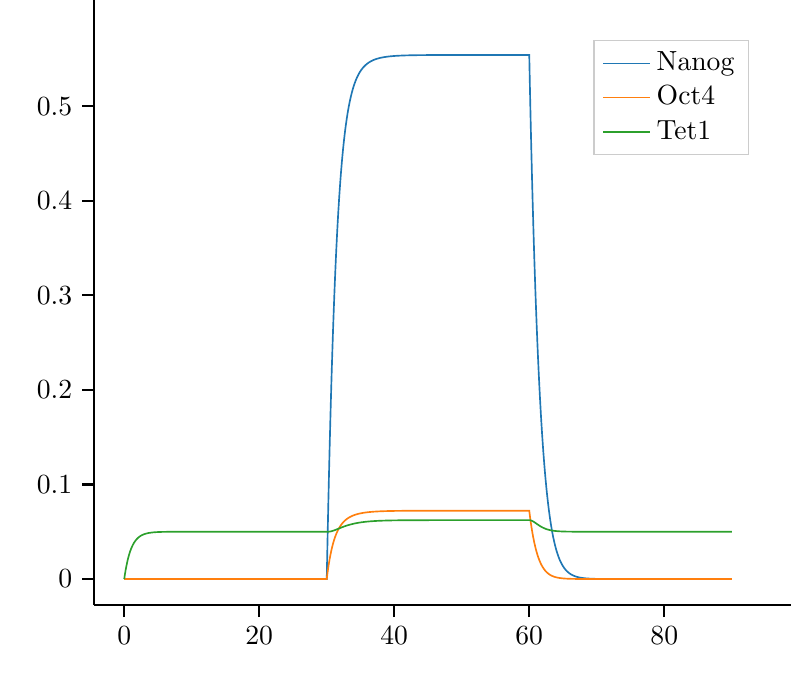
\begin{tikzpicture}

\definecolor{darkgray176}{RGB}{176,176,176}
\definecolor{darkorange25512714}{RGB}{255,127,14}
\definecolor{forestgreen4416044}{RGB}{44,160,44}
\definecolor{lightgray204}{RGB}{204,204,204}
\definecolor{steelblue31119180}{RGB}{31,119,180}

\begin{axis}[
legend cell align={left},
legend style={fill opacity=0.8, draw opacity=1, text opacity=1, draw=lightgray204},
tick align=outside,
tick pos=left,
x grid style={darkgray176},
xmin=-4.5, xmax=94.5,
xtick style={color=black},
y grid style={darkgray176},
ymin=-0.0277047168418057, ymax=0.581799053677921,
ytick style={color=black}
]
\addplot [semithick, steelblue31119180]
table {%
0 0
0.0001 0
0.0011 0
0.0111 0
0.1111 0
0.2111 0
0.3111 0
0.4111 0
0.5111 0
0.6111 0
0.7111 0
0.8111 0
0.9111 0
1.0111 0
1.1111 0
1.2111 0
1.3111 0
1.4111 0
1.5111 0
1.6111 0
1.7111 0
1.8111 0
1.9111 0
2.0111 0
2.1111 0
2.2111 0
2.3111 0
2.4111 0
2.5111 0
2.6111 0
2.7111 0
2.8111 0
2.9111 0
3.0111 0
3.1111 0
3.2111 0
3.3111 0
3.4111 0
3.5111 0
3.6111 0
3.7111 0
3.8111 0
3.9111 0
4.0111 0
4.1111 0
4.2111 0
4.3111 0
4.4111 0
4.5111 0
4.6111 0
4.7111 0
4.8111 0
4.9111 0
5.0111 0
5.1111 0
5.2111 0
5.3111 0
5.4111 0
5.5111 0
5.6111 0
5.7111 0
5.8111 0
5.9111 0
6.0111 0
6.1111 0
6.21109999999999 0
6.31109999999999 0
6.41109999999999 0
6.51109999999999 0
6.61109999999999 0
6.71109999999999 0
6.81109999999999 0
6.91109999999999 0
7.01109999999999 0
7.11109999999999 0
7.21109999999999 0
7.31109999999999 0
7.41109999999999 0
7.51109999999999 0
7.61109999999999 0
7.71109999999999 0
7.81109999999999 0
7.91109999999999 0
8.01109999999999 0
8.11109999999999 0
8.21109999999999 0
8.31109999999999 0
8.41109999999999 0
8.51109999999999 0
8.61109999999999 0
8.71109999999999 0
8.81109999999999 0
8.91109999999999 0
9.01109999999998 0
9.11109999999998 0
9.21109999999998 0
9.31109999999998 0
9.41109999999998 0
9.51109999999998 0
9.61109999999998 0
9.71109999999998 0
9.81109999999998 0
9.91109999999998 0
10.0111 0
10.1111 0
10.2111 0
10.3111 0
10.4111 0
10.5111 0
10.6111 0
10.7111 0
10.8111 0
10.9111 0
11.0111 0
11.1111 0
11.2111 0
11.3111 0
11.4111 0
11.5111 0
11.6111 0
11.7111 0
11.8111 0
11.9111 0
12.0111 0
12.1111 0
12.2111 0
12.3111 0
12.4111 0
12.5111 0
12.6111 0
12.7111 0
12.8111 0
12.9111 0
13.0111 0
13.1111 0
13.2111 0
13.3111 0
13.4111 0
13.5111 0
13.6111 0
13.7111 0
13.8111 0
13.9111 0
14.0111 0
14.1111 0
14.2111 0
14.3111 0
14.4111 0
14.5111 0
14.6111 0
14.7111 0
14.8111 0
14.9111 0
15.0111 0
15.1111 0
15.2111 0
15.3111 0
15.4111 0
15.5111 0
15.6111 0
15.7111 0
15.8111 0
15.9111 0
16.0111 0
16.1111 0
16.2111 0
16.3111 0
16.4111 0
16.5111 0
16.6111 0
16.7111 0
16.8111 0
16.9111 0
17.0111 0
17.1111 0
17.2111 0
17.3111 0
17.4111 0
17.5111 0
17.6111 0
17.7111 0
17.8111 0
17.9111 0
18.0111 0
18.1111 0
18.2111 0
18.3111 0
18.4111 0
18.5111 0
18.6111 0
18.7111 0
18.8111 0
18.9111 0
19.0111 0
19.1111 0
19.2111 0
19.3111 0
19.4111 0
19.5111 0
19.6111 0
19.7111 0
19.8111 0
19.9111 0
20.0111 0
20.1111 0
20.2111 0
20.3111 0
20.4111 0
20.5111 0
20.6111 0
20.7111 0
20.8111 0
20.9111 0
21.0111 0
21.1111 0
21.2111 0
21.3111 0
21.4111 0
21.5111 0
21.6111 0
21.7111 0
21.8111 0
21.9111 0
22.0111 0
22.1111 0
22.2111 0
22.3111 0
22.4111000000001 0
22.5111000000001 0
22.6111000000001 0
22.7111000000001 0
22.8111000000001 0
22.9111000000001 0
23.0111000000001 0
23.1111000000001 0
23.2111000000001 0
23.3111000000001 0
23.4111000000001 0
23.5111000000001 0
23.6111000000001 0
23.7111000000001 0
23.8111000000001 0
23.9111000000001 0
24.0111000000001 0
24.1111000000001 0
24.2111000000001 0
24.3111000000001 0
24.4111000000001 0
24.5111000000001 0
24.6111000000001 0
24.7111000000001 0
24.8111000000001 0
24.9111000000001 0
25.0111000000001 0
25.1111000000001 0
25.2111000000001 0
25.3111000000001 0
25.4111000000001 0
25.5111000000001 0
25.6111000000001 0
25.7111000000001 0
25.8111000000001 0
25.9111000000001 0
26.0111000000001 0
26.1111000000001 0
26.2111000000001 0
26.3111000000001 0
26.4111000000001 0
26.5111000000001 0
26.6111000000001 0
26.7111000000001 0
26.8111000000001 0
26.9111000000001 0
27.0111000000001 0
27.1111000000001 0
27.2111000000001 0
27.3111000000001 0
27.4111000000001 0
27.5111000000001 0
27.6111000000001 0
27.7111000000001 0
27.8111000000001 0
27.9111000000001 0
28.0111000000001 0
28.1111000000001 0
28.2111000000001 0
28.3111000000001 0
28.4111000000001 0
28.5111000000001 0
28.6111000000001 0
28.7111000000001 0
28.8111000000001 0
28.9111000000001 0
29.0111000000001 0
29.1111000000001 0
29.2111000000001 0
29.3111000000001 0
29.4111000000002 0
29.5111000000002 0
29.6111000000002 0
29.7111000000002 0
29.8111000000002 0
29.9111000000002 0
30 0
30 0
30.0026862579625 0.000966475201593659
30.0295488375876 0.010567234068358
30.1295488375876 0.0452583942758918
30.2295488375876 0.0782459863183292
30.3295488375876 0.109500619052527
30.4295488375876 0.139026570208306
30.5295488375876 0.166851792049081
30.6295488375876 0.193020690425914
30.7295488375876 0.217588953979675
30.8295488375876 0.240619799249135
30.9295488375876 0.262181198962019
31.0295488375876 0.282343810375518
31.1295488375876 0.301179415736205
31.2295488375876 0.318759746184408
31.3295488375876 0.335155598007197
31.4295488375876 0.350436174771917
31.5295488375876 0.36466860560323
31.6295488375876 0.377917601627168
31.7295488375876 0.390245221125059
31.8295488375876 0.401710720270754
31.9295488375876 0.41237047112841
32.0295488375876 0.422277932295939
32.1295488375876 0.431483660480442
32.2295488375876 0.440035353586978
32.3295488375876 0.447977917733376
32.4295488375876 0.45535355207523
32.5295488375876 0.462201846513969
32.6295488375876 0.468559888325358
32.7295488375876 0.474462374530762
32.8295488375876 0.479941727473967
32.9295488375876 0.485028211589717
33.0295488375876 0.489750049778177
33.1295488375876 0.494133538149691
33.2295488375876 0.498203158190562
33.3295488375876 0.501981685634416
33.4295488375876 0.505490295514357
33.5295488375876 0.508748663026133
33.6295488375876 0.51177505995804
33.7295488375876 0.514586446544533
33.8295488375876 0.517198558681618
33.9295488375876 0.519625990506542
34.0295488375876 0.521882272395065
34.1295488375876 0.523979944469026
34.2295488375876 0.525930625736958
34.3295488375876 0.527745079012968
34.4295488375876 0.529433271775202
34.5295488375876 0.531004433136221
34.6295488375876 0.532467107104467
34.7295488375876 0.533829202319443
34.8295488375876 0.535098038443998
34.9295488375876 0.536280389395756
35.0295488375876 0.537382523596626
35.1295488375876 0.538410241414986
35.2295488375876 0.539368909969778
35.3295488375876 0.54026349545966
35.4295488375876 0.541098593173781
35.5295488375876 0.541878455333807
35.6295488375876 0.542607016909716
35.7295488375876 0.543287919544664
35.8295488375876 0.543924533717059
35.9295488375876 0.544519979260855
36.0295488375876 0.54507714435817
36.1295488375876 0.545598703111519
36.2295488375876 0.546087131796448
36.3295488375876 0.546544723889063
36.4295488375876 0.546973603956909
36.5295488375876 0.547375740495893
36.6295488375876 0.547752957790511
36.7295488375877 0.5481069468694
36.8295488375877 0.548439275623359
36.9295488375877 0.548751398148331
37.0295488375877 0.549044663371476
37.1295488375877 0.54932032301437
37.2295488375877 0.549579538943474
37.3295488375877 0.549823389954468
37.4295488375877 0.550052878033602
37.5295488375877 0.550268934136091
37.6295488375877 0.550472423518643
37.7295488375877 0.550664150660419
37.8295488375877 0.550844863804205
37.9295488375877 0.551015259147173
38.0295488375877 0.551175984708377
38.1295488375877 0.551327643898112
38.2295488375877 0.551470798812309
38.3295488375877 0.551605973273394
38.4295488375877 0.551733655637378
38.5295488375877 0.551854301385433
38.6295488375877 0.551968335516794
38.7295488375877 0.552076154758519
38.8295488375877 0.552178129606429
38.9295488375877 0.552274606210448
39.0295488375877 0.552365908116507
39.1295488375877 0.552452337876245
39.2295488375877 0.552534178534844
39.3295488375877 0.552611695006528
39.4295488375877 0.552685135346514
39.5295488375877 0.552754731927481
39.6295488375877 0.552820702528038
39.7295488375877 0.552883251340014
39.8295488375877 0.552942569900922
39.9295488375877 0.552998837957391
40.0295488375877 0.553052224264933
40.1295488375877 0.553102887328979
40.2295488375877 0.553150976091724
40.3295488375877 0.553196630568956
40.4295488375877 0.553239982440734
40.5295488375877 0.553281155599452
40.6295488375877 0.55332026665855
40.7295488375877 0.55335742542489
40.8295488375877 0.553392735337559
40.9295488375877 0.553426293875649
41.0295488375877 0.553458192937364
41.1295488375877 0.553488519192621
41.2295488375877 0.553517354411134
41.3295488375877 0.553544775767816
41.4295488375877 0.553570856127204
41.5295488375877 0.553595664308447
41.6295488375877 0.553619265332316
41.7295488375877 0.553641720651544
41.8295488375877 0.553663088365731
41.9295488375877 0.553683423421933
42.0295488375877 0.553702777801989
42.1295488375877 0.553721200697518
42.2295488375877 0.553738738673509
42.3295488375877 0.553755435821292
42.4295488375877 0.553771333901656
42.5295488375877 0.553786472478819
42.6295488375877 0.553800889045876
42.7295488375877 0.553814619142345
42.8295488375877 0.553827696464337
42.9295488375877 0.553840152967876
43.0295488375877 0.553852018965838
43.1295488375877 0.553863323218934
43.2295488375877 0.553874093021158
43.3295488375877 0.553884354280061
43.4295488375877 0.553894131592195
43.5295488375877 0.553903448314066
43.6295488375877 0.553912326628873
43.7295488375877 0.553920787609321
43.8295488375878 0.55392885127676
43.9295488375878 0.553936536656889
44.0295488375878 0.553943861832249
44.1295488375878 0.553950843991701
44.2295488375878 0.553957499477092
44.3295488375878 0.553963843827278
44.4295488375878 0.553969891819667
44.5295488375878 0.553975657509448
44.6295488375878 0.553981154266638
44.7295488375878 0.553986394811079
44.8295488375878 0.553991391245523
44.9295488375878 0.553996155086902
45.0295488375878 0.554000697295908
45.1295488375878 0.554005028304975
45.2295488375878 0.554009158044759
45.3295488375878 0.554013095969202
45.4295488375878 0.55401685107927
45.5295488375878 0.554020431945437
45.6295488375878 0.554023846728976
45.7295488375878 0.554027103202152
45.8295488375878 0.554030208767353
45.9295488375878 0.55403317047523
46.0295488375878 0.554035995041909
46.1295488375878 0.554038688865304
46.2295488375878 0.554041258040612
46.3295488375878 0.554043708375005
46.4295488375878 0.554046045401586
46.5295488375878 0.55404827439263
46.6295488375878 0.554050400372168
46.7295488375878 0.55405242812793
46.8295488375878 0.5540543622227
46.9295488375878 0.554056207005097
47.0295488375878 0.554057966619821
47.1295488375878 0.554059645017402
47.2295488375878 0.554061245963451
47.3295488375878 0.554062773047468
47.4295488375878 0.554064229691215
47.5295488375878 0.554065619156677
47.6295488375878 0.554066944553631
47.7295488375878 0.554068208846857
47.8295488375878 0.554069414862988
47.9295488375878 0.554070565297033
48.0295488375878 0.554071662718582
48.1295488375878 0.554072709577717
48.2295488375878 0.554073708210631
48.3295488375878 0.554074660844981
48.4295488375878 0.554075569604984
48.5295488375878 0.554076436516268
48.6295488375878 0.554077263510495
48.7295488375878 0.554078052429756
48.8295488375878 0.554078805030763
48.9295488375878 0.554079522988837
49.0295488375878 0.554080207901716
49.1295488375878 0.554080861293168
49.2295488375878 0.554081484616443
49.3295488375878 0.554082079257561
49.4295488375878 0.554082646538443
49.5295488375878 0.554083187719891
49.6295488375878 0.554083704004435
49.7295488375878 0.55408419653904
49.8295488375878 0.554084666417687
49.9295488375878 0.554085114683836
50.0295488375878 0.554085542332768
50.1295488375878 0.554085950313824
50.2295488375878 0.554086339532531
50.3295488375878 0.554086710852635
50.4295488375878 0.55408706509804
50.5295488375878 0.554087403054645
50.6295488375878 0.554087725472114
50.7295488375878 0.554088033065546
50.8295488375879 0.554088326517073
50.9295488375879 0.554088606477393
51.0295488375879 0.554088873567214
51.1295488375879 0.554089128378646
51.2295488375879 0.55408937147652
51.3295488375879 0.554089603399649
51.4295488375879 0.554089824662031
51.5295488375879 0.554090035753992
51.6295488375879 0.55409023714328
51.7295488375879 0.554090429276107
51.8295488375879 0.554090612578144
51.9295488375879 0.554090787455466
52.0295488375879 0.554090954295458
52.1295488375879 0.554091113467675
52.2295488375879 0.554091265324668
52.3295488375879 0.554091410202762
52.4295488375879 0.554091548422808
52.5295488375879 0.554091680290895
52.6295488375879 0.55409180609903
52.7295488375879 0.554091926125787
52.8295488375879 0.554092040636927
52.9295488375879 0.554092149885984
53.0295488375879 0.554092254114835
53.1295488375879 0.554092353554228
53.2295488375879 0.554092448424303
53.3295488375879 0.554092538935076
53.4295488375879 0.554092625286902
53.5295488375879 0.554092707670929
53.6295488375879 0.55409278626951
53.7295488375879 0.554092861256619
53.8295488375879 0.554092932798228
53.9295488375879 0.554093001052679
54.0295488375879 0.554093066171035
54.1295488375879 0.554093128297415
54.2295488375879 0.554093187569312
54.3295488375879 0.554093244117899
54.4295488375879 0.55409329806832
54.5295488375879 0.554093349539964
54.6295488375879 0.554093398646736
54.7295488375879 0.554093445497304
54.8295488375879 0.55409349019534
54.9295488375879 0.554093532839753
55.0295488375879 0.554093573524905
55.1295488375879 0.554093612340823
55.2295488375879 0.554093649373394
55.3295488375879 0.55409368470456
55.4295488375879 0.554093718412495
55.5295488375879 0.554093750571784
55.6295488375879 0.55409378125358
55.7295488375879 0.55409381052577
55.8295488375879 0.55409383845312
55.9295488375879 0.554093865097418
56.0295488375879 0.554093890517616
56.1295488375879 0.554093914769956
56.2295488375879 0.554093937908093
56.3295488375879 0.554093959983221
56.4295488375879 0.554093981044177
56.5295488375879 0.554094001137558
56.6295488375879 0.554094020307818
56.7295488375879 0.554094038597367
56.8295488375879 0.55409405604667
56.9295488375879 0.55409407269433
57.0295488375879 0.554094088577176
57.1295488375879 0.554094103730348
57.2295488375879 0.554094118187367
57.3295488375879 0.554094131980217
57.4295488375879 0.554094145139411
57.5295488375879 0.554094157694062
57.6295488375879 0.554094169671943
57.7295488375879 0.554094181099552
57.829548837588 0.55409419200217
57.929548837588 0.554094202403915
58.029548837588 0.5540942123278
58.129548837588 0.554094221795776
58.229548837588 0.55409423082879
58.329548837588 0.554094239446824
58.429548837588 0.554094247668943
58.529548837588 0.554094255513336
58.629548837588 0.554094262997356
58.729548837588 0.554094270137559
58.829548837588 0.554094276949739
58.929548837588 0.554094283448968
59.029548837588 0.554094289649621
59.129548837588 0.554094295565416
59.229548837588 0.554094301209439
59.329548837588 0.554094306594176
59.429548837588 0.554094311731539
59.529548837588 0.554094316632891
59.629548837588 0.554094321309076
59.729548837588 0.554094325770437
59.829548837588 0.554094330026844
59.929548837588 0.554094334087713
60 0.554094336836115
60 0.554094336836115
60.1 0.519217851079352
60.2 0.486485001973495
60.3 0.455750564106413
60.4 0.426881474648157
60.5 0.399755711036345
60.6 0.37426126599693
60.7 0.350295207510073
60.8 0.327762814937749
60.9 0.306576785175355
61 0.286656504496648
61.1 0.267927382875405
61.2 0.250320248141545
61.3 0.2337707975115
61.4 0.218219103955644
61.5 0.20360917464192
61.6 0.189888558413901
61.7 0.17700799898875
61.8 0.164921130340018
61.9 0.153584210586534
62 0.142955890651958
62.1 0.132997013988085
62.2 0.12367044375996
62.3 0.114940914058624
62.4 0.106774901922684
62.5 0.0991405171977778
62.6 0.0920074075294885
62.7 0.0853466760589756
62.8 0.0791308096621312
62.9 0.0733336158358671
63 0.0679301665843949
63.1 0.0628967478912084
63.2 0.0582108135772548
63.3 0.0538509425418023
63.4 0.0497967985596545
63.5 0.0460290919669208
63.6000000000001 0.0425295427080117
63.7000000000001 0.0392808443395541
63.8000000000001 0.0362666286932644
63.9000000000001 0.0334714309903633
64.0000000000001 0.0308806552758349
64.1000000000001 0.0284805401028217
64.2 0.0262581244468899
64.3 0.0242012138680713
64.4 0.0222983469667868
64.5 0.0205387621993324
64.6 0.0189123651308498
64.7 0.0174096962098777
64.8 0.0160218991498454
64.9 0.0147406900003037
65 0.0135583269852367
65.1 0.0124675811782814
65.2 0.0114617080758205
65.3 0.0105344201192662
65.4 0.00967986020791307
65.5 0.00889257623386175
65.6 0.00816749666098815
65.7 0.00749990716096193
65.8 0.00688542831103798
65.8999999999999 0.00631999435084635
65.9999999999999 0.00579983298873171
66.0999999999999 0.00532144624235356
66.1999999999999 0.00488159229323899
66.2999999999999 0.00447726833074671
66.3999999999999 0.0041056943574083
66.4999999999999 0.00376429792480467
66.5999999999999 0.0034506997669534
66.6999999999999 0.00316270029656374
66.7999999999999 0.00289826692839902
66.8999999999999 0.00265552219331097
66.9999999999999 0.00243273260622044
67.0999999999999 0.00222829825135961
67.1999999999999 0.00204074304841363
67.2999999999999 0.00186870566375888
67.3999999999999 0.00171093103174942
67.4999999999999 0.00156626245191697
67.5999999999999 0.00143363422898949
67.6999999999998 0.00131206482377028
67.7999999999998 0.00120065048412955
67.8999999999998 0.00109855932661997
67.9999999999998 0.00100502584051956
68.0999999999998 0.000919345787412942
68.1999999999998 0.000840871470731025
68.2999999999998 0.000769007350969988
68.3999999999998 0.000703205983591837
68.4999999999998 0.000642964257864339
68.5999999999998 0.000587819916121114
68.6999999999998 0.000537348334108354
68.7999999999998 0.000491159544229377
68.8999999999998 0.000448895484599286
68.9999999999998 0.000410227457877469
69.0999999999998 0.00037485378485446
69.1999999999998 0.000342497638731194
69.2999999999998 0.00031290504694286
69.3999999999997 0.000285843048246816
69.4999999999997 0.000261097993615038
69.5999999999997 0.000238473980247348
69.6999999999997 0.000217791408753416
69.7999999999997 0.000198885654240644
69.8999999999997 0.000181605842693
69.9999999999997 0.000165813724634347
70.0999999999997 0.000151382638640394
70.1999999999997 0.000138196557797855
70.2999999999997 0.000126149212709453
70.3999999999997 0.000115143285110699
70.4999999999997 0.000105089666600732
70.5999999999997 9.59067773964878e-05
70.6999999999997 8.75199403987748e-05
70.7999999999997 7.98608062120337e-05
70.8999999999997 7.28668250881882e-05
70.9999999999997 6.64807620705399e-05
71.0999999999997 6.06502518975309e-05
71.1999999999996 5.53273904897645e-05
71.2999999999996 5.04683600882212e-05
71.3999999999996 4.60330853383793e-05
71.4999999999996 4.19849178251042e-05
71.5999999999996 3.82903467578288e-05
71.6999999999996 3.49187336857459e-05
71.7999999999996 3.18420692894731e-05
71.8999999999996 2.90347504498471e-05
71.9999999999996 2.64733759370505e-05
72.0999999999996 2.41365591949789e-05
72.1999999999996 2.20047568174017e-05
72.2999999999996 2.00601114247659e-05
72.3999999999996 1.82863077541366e-05
72.4999999999996 1.66684408703651e-05
72.5999999999996 1.519289549474e-05
72.6999999999996 1.38472355286498e-05
72.7999999999996 1.26201029246711e-05
72.8999999999996 1.15011251264957e-05
72.9999999999995 1.04808303626408e-05
73.0999999999995 9.55057013738404e-06
73.1999999999995 8.70244831620153e-06
73.2999999999995 7.92925625252233e-06
73.3999999999995 7.22441344818025e-06
73.4999999999995 6.58191328184642e-06
73.5999999999995 5.99627337825139e-06
73.6999999999995 5.46249022641584e-06
73.7999999999995 4.97599768764807e-06
73.8999999999995 4.53262906396087e-06
73.9999999999995 4.12858242501802e-06
74.0999999999995 3.76038891693512e-06
74.1999999999995 3.42488379940886e-06
74.2999999999995 3.11917997889781e-06
74.3999999999995 2.84064382507844e-06
74.4999999999995 2.58687307569282e-06
74.5999999999995 2.35567665131852e-06
74.6999999999994 2.14505621664627e-06
74.7999999999994 1.95318933865658e-06
74.8999999999994 1.77841410474486e-06
74.9999999999994 1.61921507544807e-06
75.0999999999994 1.47421045706167e-06
75.1999999999994 1.34214038918191e-06
75.2999999999994 1.22185625113883e-06
75.3999999999994 1.11231089946635e-06
75.4999999999994 1.01254975604987e-06
75.5999999999994 9.21702673454483e-07
75.6999999999994 8.38976510221925e-07
75.7999999999994 7.63648354678151e-07
75.8999999999994 6.95059341061153e-07
75.9999999999994 6.32609006600212e-07
76.0999999999994 5.75750142590524e-07
76.1999999999994 5.23984096545288e-07
76.2999999999994 4.7685648620207e-07
76.3999999999994 4.33953289540561e-07
76.4999999999993 3.94897278060866e-07
76.5999999999993 3.59344763399711e-07
76.6999999999993 3.26982629948383e-07
76.7999999999993 2.97525628501468e-07
76.8999999999993 2.70713908128011e-07
76.9999999999993 2.46310765433875e-07
77.0999999999993 2.24100592191446e-07
77.1999999999993 2.03887003964885e-07
77.2999999999993 1.85491133869006e-07
77.3999999999993 1.6875007697972e-07
77.4999999999993 1.53515472174832e-07
77.5999999999993 1.39652209336023e-07
77.6999999999993 1.27037250895374e-07
77.7999999999993 1.15558557671241e-07
77.8999999999993 1.05114109816585e-07
77.9999999999993 9.56110145049981e-08
78.0999999999993 8.69646927122717e-08
78.1999999999992 7.90981381203524e-08
78.2999999999992 7.19412417814244e-08
78.3999999999992 6.54301767376115e-08
78.4999999999992 5.95068373010239e-08
78.5999999999992 5.41183281637423e-08
78.6999999999992 4.92164989316817e-08
78.7999999999992 4.47575200636062e-08
78.8999999999992 4.0701496550074e-08
78.9999999999992 3.7012115989716e-08
79.0999999999992 3.36563280146612e-08
79.1999999999992 3.06040522855689e-08
79.2999999999992 2.78279125218503e-08
79.3999999999992 2.53029942562993e-08
79.4999999999992 2.30066242073814e-08
79.5999999999992 2.09181693485511e-08
79.6999999999992 1.90188539237415e-08
79.7999999999992 1.72915928130326e-08
79.8999999999992 1.57208397937375e-08
79.9999999999991 1.42924493709623e-08
80.0999999999991 1.29935509691617e-08
80.1999999999991 1.18124343833328e-08
80.2999999999991 1.07384454861649e-08
80.3999999999991 9.76189127652446e-09
80.4999999999991 8.8739534358505e-09
80.5999999999991 8.06660963306426e-09
80.6999999999991 7.33256188608224e-09
80.7999999999991 6.66517134953927e-09
80.8999999999991 6.05839895440463e-09
80.9999999999991 5.50675137628546e-09
81.0999999999991 5.00523185579699e-09
81.1999999999991 4.54929543683582e-09
81.2999999999991 4.13480822728451e-09
81.3999999999991 3.75801032193637e-09
81.4999999999991 3.41548205955927e-09
81.5999999999991 3.1041133152949e-09
81.6999999999991 2.82107555626595e-09
81.799999999999 2.56379641256879e-09
81.899999999999 2.32993653797245e-09
81.999999999999 2.1173685548183e-09
82.099999999999 1.92415789599208e-09
82.199999999999 1.74854537358092e-09
82.299999999999 1.58893131907733e-09
82.399999999999 1.44386115388196e-09
82.499999999999 1.31201226150825e-09
82.599999999999 1.1921820444148e-09
82.699999999999 1.08327705888506e-09
82.799999999999 9.84303130931234e-10
82.899999999999 8.94356364902453e-10
82.999999999999 8.12614964402606e-10
83.099999999999 7.38331792340216e-10
83.199999999999 6.70827603504004e-10
83.299999999999 6.09484889041153e-10
83.399999999999 5.53742277663019e-10
83.4999999999989 5.03089443362949e-10
83.5999999999989 4.57062473946415e-10
83.6999999999989 4.15239658784578e-10
83.7999999999989 3.77237657944704e-10
83.8999999999989 3.42708018257597e-10
83.9999999999989 3.11334004983224e-10
84.0999999999989 2.82827720558462e-10
84.1999999999989 2.56927484480199e-10
84.2999999999989 2.3339545071552e-10
84.3999999999989 2.12015441159182e-10
84.4999999999989 1.92590975595661e-10
84.5999999999989 1.74943480386038e-10
84.6999999999989 1.589106597044e-10
84.7999999999989 1.44345014608464e-10
84.8999999999989 1.31112496557799e-10
84.9999999999989 1.19091283202075e-10
85.0999999999989 1.0817066536188e-10
85.1999999999989 9.82500351257375e-11
85.2999999999988 8.92379658977732e-11
85.3999999999988 8.1051376059212e-11
85.4999999999988 7.36147686609086e-11
85.5999999999988 6.68595402501011e-11
85.6999999999988 6.07233525586874e-11
85.7999999999988 5.51495613481017e-11
85.8999999999988 5.00866972223921e-11
85.9999999999988 4.54879936909748e-11
86.0999999999988 4.13109581899772e-11
86.1999999999988 3.75169821598928e-11
86.2999999999988 3.40709866309458e-11
86.3999999999988 3.0941100089257e-11
86.4999999999988 2.80983656895137e-11
86.5999999999988 2.55164751459815e-11
86.6999999999988 2.31715268757559e-11
86.7999999999988 2.10418061883042e-11
86.8999999999988 1.91075855155669e-11
86.9999999999987 1.73509428589831e-11
87.0999999999987 1.57555967953981e-11
87.1999999999987 1.43067565344122e-11
87.2999999999987 1.2990985656674e-11
87.3999999999987 1.17960782871587e-11
87.4999999999987 1.07109465707161e-11
87.5999999999987 9.72551842014575e-12
87.6999999999987 8.83064460069138e-12
87.7999999999987 8.01801429998405e-12
87.8999999999987 7.28007840987436e-12
87.9999999999987 6.60997981697905e-12
88.0999999999987 6.00149006276056e-12
88.1999999999987 5.44895179214017e-12
88.2999999999987 4.94722646254212e-12
88.3999999999987 4.49164683335703e-12
88.4999999999987 4.07797379953295e-12
88.5999999999987 3.70235717274883e-12
88.6999999999987 3.36130004975745e-12
88.7999999999986 3.05162644033173e-12
88.8999999999986 2.77045185710714e-12
88.9999999999986 2.51515659675553e-12
89.0999999999986 2.2833614665981e-12
89.1999999999986 2.07290573319265e-12
89.2999999999986 1.8818270898149e-12
89.3999999999986 1.70834345828367e-12
89.4999999999986 1.55083645742066e-12
89.5999999999986 1.40783638574368e-12
89.6999999999986 1.27800857990468e-12
89.7999999999986 1.16014102302948e-12
89.8999999999986 1.05313308860792e-12
89.9999999999986 9.55985316028894e-13
90 9.5598531602758e-13
};
\addlegendentry{Nanog}
\addplot [semithick, darkorange25512714]
table {%
0 0
0.0001 0
0.0011 0
0.0111 0
0.1111 0
0.2111 0
0.3111 0
0.4111 0
0.5111 0
0.6111 0
0.7111 0
0.8111 0
0.9111 0
1.0111 0
1.1111 0
1.2111 0
1.3111 0
1.4111 0
1.5111 0
1.6111 0
1.7111 0
1.8111 0
1.9111 0
2.0111 0
2.1111 0
2.2111 0
2.3111 0
2.4111 0
2.5111 0
2.6111 0
2.7111 0
2.8111 0
2.9111 0
3.0111 0
3.1111 0
3.2111 0
3.3111 0
3.4111 0
3.5111 0
3.6111 0
3.7111 0
3.8111 0
3.9111 0
4.0111 0
4.1111 0
4.2111 0
4.3111 0
4.4111 0
4.5111 0
4.6111 0
4.7111 0
4.8111 0
4.9111 0
5.0111 0
5.1111 0
5.2111 0
5.3111 0
5.4111 0
5.5111 0
5.6111 0
5.7111 0
5.8111 0
5.9111 0
6.0111 0
6.1111 0
6.21109999999999 0
6.31109999999999 0
6.41109999999999 0
6.51109999999999 0
6.61109999999999 0
6.71109999999999 0
6.81109999999999 0
6.91109999999999 0
7.01109999999999 0
7.11109999999999 0
7.21109999999999 0
7.31109999999999 0
7.41109999999999 0
7.51109999999999 0
7.61109999999999 0
7.71109999999999 0
7.81109999999999 0
7.91109999999999 0
8.01109999999999 0
8.11109999999999 0
8.21109999999999 0
8.31109999999999 0
8.41109999999999 0
8.51109999999999 0
8.61109999999999 0
8.71109999999999 0
8.81109999999999 0
8.91109999999999 0
9.01109999999998 0
9.11109999999998 0
9.21109999999998 0
9.31109999999998 0
9.41109999999998 0
9.51109999999998 0
9.61109999999998 0
9.71109999999998 0
9.81109999999998 0
9.91109999999998 0
10.0111 0
10.1111 0
10.2111 0
10.3111 0
10.4111 0
10.5111 0
10.6111 0
10.7111 0
10.8111 0
10.9111 0
11.0111 0
11.1111 0
11.2111 0
11.3111 0
11.4111 0
11.5111 0
11.6111 0
11.7111 0
11.8111 0
11.9111 0
12.0111 0
12.1111 0
12.2111 0
12.3111 0
12.4111 0
12.5111 0
12.6111 0
12.7111 0
12.8111 0
12.9111 0
13.0111 0
13.1111 0
13.2111 0
13.3111 0
13.4111 0
13.5111 0
13.6111 0
13.7111 0
13.8111 0
13.9111 0
14.0111 0
14.1111 0
14.2111 0
14.3111 0
14.4111 0
14.5111 0
14.6111 0
14.7111 0
14.8111 0
14.9111 0
15.0111 0
15.1111 0
15.2111 0
15.3111 0
15.4111 0
15.5111 0
15.6111 0
15.7111 0
15.8111 0
15.9111 0
16.0111 0
16.1111 0
16.2111 0
16.3111 0
16.4111 0
16.5111 0
16.6111 0
16.7111 0
16.8111 0
16.9111 0
17.0111 0
17.1111 0
17.2111 0
17.3111 0
17.4111 0
17.5111 0
17.6111 0
17.7111 0
17.8111 0
17.9111 0
18.0111 0
18.1111 0
18.2111 0
18.3111 0
18.4111 0
18.5111 0
18.6111 0
18.7111 0
18.8111 0
18.9111 0
19.0111 0
19.1111 0
19.2111 0
19.3111 0
19.4111 0
19.5111 0
19.6111 0
19.7111 0
19.8111 0
19.9111 0
20.0111 0
20.1111 0
20.2111 0
20.3111 0
20.4111 0
20.5111 0
20.6111 0
20.7111 0
20.8111 0
20.9111 0
21.0111 0
21.1111 0
21.2111 0
21.3111 0
21.4111 0
21.5111 0
21.6111 0
21.7111 0
21.8111 0
21.9111 0
22.0111 0
22.1111 0
22.2111 0
22.3111 0
22.4111000000001 0
22.5111000000001 0
22.6111000000001 0
22.7111000000001 0
22.8111000000001 0
22.9111000000001 0
23.0111000000001 0
23.1111000000001 0
23.2111000000001 0
23.3111000000001 0
23.4111000000001 0
23.5111000000001 0
23.6111000000001 0
23.7111000000001 0
23.8111000000001 0
23.9111000000001 0
24.0111000000001 0
24.1111000000001 0
24.2111000000001 0
24.3111000000001 0
24.4111000000001 0
24.5111000000001 0
24.6111000000001 0
24.7111000000001 0
24.8111000000001 0
24.9111000000001 0
25.0111000000001 0
25.1111000000001 0
25.2111000000001 0
25.3111000000001 0
25.4111000000001 0
25.5111000000001 0
25.6111000000001 0
25.7111000000001 0
25.8111000000001 0
25.9111000000001 0
26.0111000000001 0
26.1111000000001 0
26.2111000000001 0
26.3111000000001 0
26.4111000000001 0
26.5111000000001 0
26.6111000000001 0
26.7111000000001 0
26.8111000000001 0
26.9111000000001 0
27.0111000000001 0
27.1111000000001 0
27.2111000000001 0
27.3111000000001 0
27.4111000000001 0
27.5111000000001 0
27.6111000000001 0
27.7111000000001 0
27.8111000000001 0
27.9111000000001 0
28.0111000000001 0
28.1111000000001 0
28.2111000000001 0
28.3111000000001 0
28.4111000000001 0
28.5111000000001 0
28.6111000000001 0
28.7111000000001 0
28.8111000000001 0
28.9111000000001 0
29.0111000000001 0
29.1111000000001 0
29.2111000000001 0
29.3111000000001 0
29.4111000000002 0
29.5111000000002 0
29.6111000000002 0
29.7111000000002 0
29.8111000000002 0
29.9111000000002 0
30 0
30 0
30.0026862579625 0.000160959192932928
30.0295488375876 0.00174700466258397
30.1295488375876 0.00729368481827424
30.2295488375876 0.0123289305767425
30.3295488375876 0.0169149747621551
30.4295488375876 0.021102923870268
30.5295488375876 0.0249346852800907
30.6295488375876 0.0284454622466816
30.7295488375876 0.031665564913883
30.8295488375876 0.0346215909725772
30.9295488375876 0.037337190862689
31.0295488375876 0.0398335800903369
31.1295488375876 0.0421298993857418
31.2295488375876 0.0442434817931022
31.3295488375876 0.0461900610086228
31.4295488375876 0.0479839410552
31.5295488375876 0.0496381392574179
31.6295488375876 0.0511645098105133
31.7295488375876 0.0525738525208938
31.8295488375876 0.0538760096931989
31.9295488375876 0.0550799531778107
32.0295488375876 0.0561938630057026
32.1295488375876 0.0572251986712339
32.2295488375876 0.0581807638890017
32.3295488375876 0.059066765495964
32.4295488375876 0.0598888670637878
32.5295488375876 0.0606522377102389
32.6295488375876 0.0613615965412508
32.7295488375876 0.0620212531102943
32.8295488375876 0.0626351442446891
32.9295488375876 0.0632068675569978
33.0295488375876 0.0637397119320619
33.1295488375876 0.0642366852555844
33.2295488375876 0.064700539627836
33.3295488375876 0.0651337942856456
33.4295488375876 0.0655387564370789
33.5295488375876 0.0659175401959299
33.6295488375876 0.0662720837872018
33.7295488375876 0.0666041651800496
33.8295488375876 0.066915416291093
33.9295488375876 0.0672073358885153
34.0295488375876 0.0674813013158713
34.1295488375876 0.0677385791439666
34.2295488375876 0.0679803348494756
34.3295488375876 0.068207641610087
34.4295488375876 0.0684214882978304
34.5295488375876 0.0686227867448049
34.6295488375876 0.0688123783487389
34.7295488375876 0.0689910400796149
34.8295488375876 0.0691594899429424
34.9295488375876 0.0693183919501205
35.0295488375876 0.0694683606416448
35.1295488375876 0.0696099652046581
35.2295488375876 0.0697437332224686
35.3295488375876 0.0698701540901474
35.4295488375876 0.0699896821271197
35.5295488375876 0.0701027394147685
35.6295488375876 0.0702097183844404
35.7295488375876 0.0703109841788579
35.8295488375876 0.0704068768077836
35.9295488375876 0.0704977131168207
36.0295488375876 0.0705837885864629
36.1295488375876 0.0706653789768947
36.2295488375876 0.070742741832593
36.3295488375876 0.0708161178594578
36.4295488375876 0.0708857321860097
36.5295488375876 0.0709517955191088
36.6295488375876 0.0710145052036743
36.7295488375877 0.0710740461949957
36.8295488375877 0.0711305919514291
36.9295488375877 0.0711843052545419
37.0295488375877 0.0712353389631178
37.1295488375877 0.0712838367068365
37.2295488375877 0.0713299335249054
37.3295488375877 0.0713737564544351
37.4295488375877 0.0714154250729072
37.5295488375877 0.0714550519986872
37.6295488375877 0.0714927433531707
37.7295488375877 0.0715285991878258
37.8295488375877 0.0715627138790984
37.9295488375877 0.0715951764938777
38.0295488375877 0.0716260711279756
38.1295488375877 0.0716554772198559
38.2295488375877 0.0716834698416462
38.3295488375877 0.0717101199692853
38.4295488375877 0.0717354947334975
38.5295488375877 0.0717596576531312
38.6295488375877 0.0717826688522684
38.7295488375877 0.0718045852623867
38.8295488375877 0.0718254608107456
38.9295488375877 0.0718453465960659
39.0295488375877 0.0718642910524821
39.1295488375877 0.0718823401026602
39.2295488375877 0.0718995373009021
39.3295488375877 0.071915923966985
39.4295488375877 0.0719315393114241
39.5295488375877 0.0719464205527877
39.6295488375877 0.0719606030276439
39.7295488375877 0.071974120293669
39.8295488375877 0.0719870042264061
39.9295488375877 0.0719992851101215
40.0295488375877 0.0720109917231721
40.1295488375877 0.0720221514182635
40.2295488375877 0.0720327901979485
40.3295488375877 0.0720429327856893
40.4295488375877 0.0720526026927803
40.5295488375877 0.0720618222814073
40.6295488375877 0.0720706128240962
40.7295488375877 0.0720789945597879
40.8295488375877 0.0720869867467537
40.9295488375877 0.0720946077125567
41.0295488375877 0.0721018749012421
41.1295488375877 0.0721088049179318
41.2295488375877 0.0721154135709838
41.3295488375877 0.0721217159118643
41.4295488375877 0.0721277262728735
41.5295488375877 0.0721334583028526
41.6295488375877 0.072138925000993
41.7295488375877 0.0721441387488595
41.8295488375877 0.0721491113407325
41.9295488375877 0.0721538540123664
42.0295488375877 0.0721583774682552
42.1295488375877 0.0721626919074905
42.2295488375877 0.0721668070482921
42.3295488375877 0.0721707321512845
42.4295488375877 0.0721744760415906
42.5295488375877 0.0721780471298066
42.6295488375877 0.0721814534319205
42.7295488375877 0.0721847025882308
42.8295488375877 0.0721878018813207
42.9295488375877 0.0721907582531368
43.0295488375877 0.0721935783212219
43.1295488375877 0.0721962683941455
43.2295488375877 0.0721988344861749
43.3295488375877 0.072201282331226
43.4295488375877 0.0722036173961322
43.5295488375877 0.0722058448932665
43.6295488375877 0.0722079697925488
43.7295488375877 0.0722099968328727
43.8295488375878 0.072211930532978
43.9295488375878 0.0722137752017998
44.0295488375878 0.0722155349483192
44.1295488375878 0.0722172136909416
44.2295488375878 0.0722188151664246
44.3295488375878 0.0722203429383802
44.4295488375878 0.072221800405371
44.5295488375878 0.0722231908086204
44.6295488375878 0.0722245172393569
44.7295488375878 0.0722257826458097
44.8295488375878 0.0722269898398724
44.9295488375878 0.0722281415034524
45.0295488375878 0.0722292401945198
45.1295488375878 0.0722302883528705
45.2295488375878 0.0722312883056193
45.3295488375878 0.0722322422724327
45.4295488375878 0.0722331523705179
45.5295488375878 0.0722340206193754
45.6295488375878 0.0722348489453309
45.7295488375878 0.0722356391858533
45.8295488375878 0.0722363930936717
45.9295488375878 0.0722371123406997
46.0295488375878 0.0722377985217759
46.1295488375878 0.0722384531582307
46.2295488375878 0.0722390777012862
46.3295488375878 0.0722396735352977
46.4295488375878 0.072240241980845
46.5295488375878 0.0722407842976786
46.6295488375878 0.0722413016875303
46.7295488375878 0.0722417952967922
46.8295488375878 0.0722422662190715
46.9295488375878 0.0722427154976275
47.0295488375878 0.072243144127694
47.1295488375878 0.072243553058696
47.2295488375878 0.0722439431963615
47.3295488375878 0.0722443154047374
47.4295488375878 0.0722446705081109
47.5295488375878 0.0722450092928425
47.6295488375878 0.0722453325091136
47.7295488375878 0.0722456408725942
47.8295488375878 0.0722459350660326
47.9295488375878 0.0722462157407722
48.0295488375878 0.072246483518198
48.1295488375878 0.0722467389911161
48.2295488375878 0.07224698272507
48.3295488375878 0.0722472152595957
48.4295488375878 0.0722474371094191
48.5295488375878 0.0722476487655979
48.6295488375878 0.072247850696611
48.7295488375878 0.0722480433493979
48.8295488375878 0.0722482271503496
48.9295488375878 0.0722484025062543
49.0295488375878 0.0722485698051994
49.1295488375878 0.0722487294174316
49.2295488375878 0.0722488816961778
49.3295488375878 0.0722490269784283
49.4295488375878 0.072249165585683
49.5295488375878 0.0722492978246643
49.6295488375878 0.0722494239879968
49.7295488375878 0.0722495443548553
49.8295488375878 0.0722496591915837
49.9295488375878 0.0722497687522845
50.0295488375878 0.0722498732793824
50.1295488375878 0.0722499730041604
50.2295488375878 0.0722500681472727
50.3295488375878 0.0722501589192331
50.4295488375878 0.0722502455208812
50.5295488375878 0.0722503281438273
50.6295488375878 0.0722504069708763
50.7295488375878 0.072250482176433
50.8295488375879 0.0722505539268876
50.9295488375879 0.0722506223809848
51.0295488375879 0.0722506876901745
51.1295488375879 0.0722507499989477
51.2295488375879 0.072250809445156
51.3295488375879 0.0722508661603168
51.4295488375879 0.0722509202699045
51.5295488375879 0.0722509718936281
51.6295488375879 0.0722510211456963
51.7295488375879 0.0722510681350703
51.8295488375879 0.0722511129657047
51.9295488375879 0.0722511557367779
52.0295488375879 0.0722511965429112
52.1295488375879 0.0722512354743789
52.2295488375879 0.072251272617307
52.3295488375879 0.072251308053865
52.4295488375879 0.0722513418624467
52.5295488375879 0.0722513741178443
52.6295488375879 0.0722514048914137
52.7295488375879 0.0722514342512326
52.8295488375879 0.0722514622622506
52.9295488375879 0.0722514889864335
53.0295488375879 0.0722515144829002
53.1295488375879 0.0722515388080534
53.2295488375879 0.0722515620157045
53.3295488375879 0.0722515841571926
53.4295488375879 0.0722516052814983
53.5295488375879 0.0722516254353518
53.6295488375879 0.0722516446633364
53.7295488375879 0.0722516630079872
53.8295488375879 0.0722516805098851
53.9295488375879 0.0722516972077467
54.0295488375879 0.0722517131385097
54.1295488375879 0.0722517283374151
54.2295488375879 0.0722517428380847
54.3295488375879 0.0722517566725957
54.4295488375879 0.0722517698715516
54.5295488375879 0.0722517824641501
54.6295488375879 0.0722517944782472
54.7295488375879 0.0722518059404195
54.8295488375879 0.0722518168760224
54.9295488375879 0.0722518273092467
55.0295488375879 0.0722518372631716
55.1295488375879 0.0722518467598161
55.2295488375879 0.0722518558201878
55.3295488375879 0.0722518644643289
55.4295488375879 0.0722518727113612
55.5295488375879 0.0722518805795277
55.6295488375879 0.0722518880862335
55.7295488375879 0.072251895248084
55.8295488375879 0.0722519020809219
55.9295488375879 0.0722519085998619
56.0295488375879 0.0722519148193245
56.1295488375879 0.0722519207530675
56.2295488375879 0.0722519264142169
56.3295488375879 0.0722519318152956
56.4295488375879 0.0722519369682511
56.5295488375879 0.0722519418844821
56.6295488375879 0.0722519465748637
56.7295488375879 0.0722519510497713
56.8295488375879 0.0722519553191038
56.9295488375879 0.0722519593923051
57.0295488375879 0.0722519632783856
57.1295488375879 0.0722519669859414
57.2295488375879 0.0722519705231739
57.3295488375879 0.0722519738979077
57.4295488375879 0.0722519771176079
57.5295488375879 0.0722519801893967
57.6295488375879 0.0722519831200691
57.7295488375879 0.0722519859161079
57.829548837588 0.0722519885836982
57.929548837588 0.0722519911287407
58.029548837588 0.0722519935568653
58.129548837588 0.0722519958734432
58.229548837588 0.0722519980835987
58.329548837588 0.0722520001922208
58.429548837588 0.072252002203974
58.529548837588 0.0722520041233083
58.629548837588 0.0722520059544694
58.729548837588 0.072252007701508
58.829548837588 0.0722520093682886
58.929548837588 0.0722520109584982
59.029548837588 0.0722520124756544
59.129548837588 0.0722520139231134
59.229548837588 0.0722520153040768
59.329548837588 0.0722520166215996
59.429548837588 0.0722520178785961
59.529548837588 0.0722520190778469
59.629548837588 0.0722520202220048
59.729548837588 0.0722520213136007
59.829548837588 0.0722520223550494
59.929548837588 0.0722520233486544
60 0.0722520240211281
60 0.0722520240211281
60.1 0.0664900786004402
60.2 0.0611760249780536
60.3 0.0562713251192646
60.4 0.0517419053285664
60.5 0.0475575042284112
60.6 0.0436911076937085
60.7 0.0401184645051677
60.8 0.0368176755685557
60.9 0.0337688490081555
61 0.0309538132482681
61.1 0.0283558803008975
61.2 0.0259596518261944
61.3 0.0237508610656505
61.4 0.0217162444072296
61.5 0.0198434370713938
61.6 0.0181208881592448
61.7 0.0165377910396618
61.8 0.0150840257420515
61.9 0.0137501106453279
62 0.0125271613007912
62.1 0.011406854692636
62.2 0.010381397626506
62.3 0.0094434982494964
62.4 0.00858633995258519
62.5 0.00780355709833167
62.6 0.00708921216282201
62.7 0.00643777399082768
62.8 0.00584409694551049
62.9 0.00530340079592783
63 0.00481125123273403
63.1 0.00436354093903656
63.2 0.00395647117224249
63.3 0.00358653383575949
63.4 0.00325049403766381
63.5 0.00294537314749294
63.6000000000001 0.00266843237248302
63.7000000000001 0.00241715688109713
63.8000000000001 0.00218924050485989
63.9000000000001 0.00198257104969475
64.0000000000001 0.00179521624561641
64.1000000000001 0.00162541035929384
64.2 0.00147154148823348
64.3 0.00133213954868821
64.4 0.00120586496237826
64.5 0.00109149804014532
64.6 0.000987929054089359
64.7 0.000894148983807204
64.8 0.000809240917222691
64.9 0.000732372082252753
65 0.000662786482211293
65.1 0.000599798105384146
65.2 0.000542784677549465
65.3 0.000491181925282703
65.4 0.000444478317576251
65.5 0.000402210253519747
65.6 0.000363957664429429
65.7 0.000329339999791982
65.8 0.000298012567617087
65.8999999999999 0.000269663201201206
65.9999999999999 0.000244009225831144
66.0999999999999 0.000220794700548469
66.1999999999999 0.00019978791171326
66.2999999999999 0.000180779096714943
66.3999999999999 0.000163578377753761
66.4999999999999 0.000148013887139884
66.5999999999999 0.000133930067014684
66.6999999999999 0.00012118612778134
66.7999999999999 0.000109654650834207
66.8999999999999 9.92203223956067e-05
66.9999999999999 8.97787864045127e-05
67.0999999999999 8.12356054550941e-05
67.1999999999999 7.35053197568219e-05
67.2999999999999 6.65105949849402e-05
67.3999999999999 6.0181450714526e-05
67.4999999999999 5.44545618872266e-05
67.5999999999999 4.92726264514578e-05
67.6999999999998 4.45837929487687e-05
67.7999999999998 4.03411423955791e-05
67.8999999999998 3.65022193347984e-05
67.9999999999998 3.30286074099902e-05
68.0999999999998 2.98855452496036e-05
68.1999999999998 2.7041578843969e-05
68.2999999999998 2.44682469566445e-05
68.3999999999998 2.2139796437448e-05
68.4999999999998 2.00329246000446e-05
68.5999999999998 1.81265460949673e-05
68.6999999999998 1.64015819519216e-05
68.7999999999998 1.48407686854261e-05
68.8999999999998 1.34284855573611e-05
68.9999999999998 1.21505982707418e-05
69.0999999999998 1.09943175327359e-05
69.1999999999998 9.94807107318943e-06
69.2999999999998 9.00138783916221e-06
69.3999999999997 8.14479320750223e-06
69.4999999999997 7.36971416750953e-06
69.5999999999997 6.66839352533267e-06
69.6999999999997 6.03381227188727e-06
69.7999999999997 5.45961933767864e-06
69.8999999999997 4.94006803175643e-06
69.9999999999997 4.4699585288628e-06
70.0999999999997 4.04458582931874e-06
70.1999999999997 3.65969267092953e-06
70.2999999999997 3.31142692172371e-06
70.3999999999997 2.99630302716427e-06
70.4999999999997 2.71116712603321e-06
70.5999999999997 2.45316548589575e-06
70.6999999999997 2.21971594226447e-06
70.7999999999997 2.00848205563903e-06
70.8999999999997 1.81734972779271e-06
70.9999999999997 1.64440604328653e-06
71.0999999999997 1.48792012445891e-06
71.1999999999996 1.34632580828854e-06
71.2999999999996 1.21820597175997e-06
71.3999999999996 1.10227834885906e-06
71.4999999999996 9.9738269725307e-07
71.5999999999996 9.02469186217609e-07
71.6999999999996 8.16587889594593e-07
71.7999999999996 7.38879278624599e-07
71.8999999999996 6.68565619503669e-07
71.9999999999996 6.04943189569185e-07
72.0999999999996 5.47375234212361e-07
72.1999999999996 4.9528559402819e-07
72.2999999999996 4.4815293842156e-07
72.3999999999996 4.0550554795777e-07
72.4999999999996 3.66916593237641e-07
72.5999999999996 3.31999863046761e-07
72.6999999999996 3.00405899024848e-07
72.7999999999996 2.7181849816979e-07
72.8999999999996 2.45951548172297e-07
72.9999999999995 2.22546163908181e-07
73.0999999999995 2.01368096429355e-07
73.1999999999995 1.82205388521878e-07
73.2999999999995 1.64866253367107e-07
73.3999999999995 1.49177155074907e-07
73.4999999999995 1.34981071878242e-07
73.5999999999995 1.22135924606645e-07
73.6999999999995 1.10513154710188e-07
73.7999999999995 9.99964376023597e-08
73.8999999999995 9.04805184445421e-08
73.9999999999995 8.18701587202421e-08
74.0999999999995 7.4079183056031e-08
74.1999999999995 6.70296167494623e-08
74.2999999999995 6.06509053720574e-08
74.3999999999995 5.48792086368829e-08
74.4999999999995 4.96567614635121e-08
74.5999999999995 4.49312958456926e-08
74.6999999999994 4.06555177355784e-08
74.7999999999994 3.6786633709009e-08
74.8999999999994 3.3285922674541e-08
74.9999999999994 3.01183483397553e-08
75.0999999999994 2.72522085562687e-08
75.1999999999994 2.46588180339811e-08
75.2999999999994 2.2312221249053e-08
75.3999999999994 2.01889326723008e-08
75.4999999999994 1.82677017181293e-08
75.5999999999994 1.65293000615299e-08
75.6999999999994 1.49563291945426e-08
75.7999999999994 1.35330462961415e-08
75.8999999999994 1.22452066727922e-08
75.9999999999994 1.1079921192772e-08
76.0999999999994 1.0025527287408e-08
76.1999999999994 9.07147222817127e-09
76.2999999999994 8.20820751142297e-09
76.3999999999994 7.4270932937817e-09
76.4999999999993 6.72031192166735e-09
76.5999999999993 6.08078968959705e-09
76.6999999999993 5.50212604416357e-09
76.7999999999993 4.97852952514604e-09
76.8999999999993 4.50475980262978e-09
76.9999999999993 4.07607523002358e-09
77.0999999999993 3.6881853880672e-09
77.1999999999993 3.33720814487361e-09
77.2999999999993 3.01963080224853e-09
77.3999999999993 2.73227493942647e-09
77.4999999999993 2.47226460236758e-09
77.5999999999993 2.23699752024322e-09
77.6999999999993 2.02411906103499e-09
77.7999999999993 1.83149866558623e-09
77.8999999999993 1.65720852425002e-09
77.9999999999993 1.4995042827224e-09
78.0999999999993 1.35680758395833e-09
78.1999999999992 1.22769027144396e-09
78.2999999999992 1.11086009572631e-09
78.3999999999992 1.00514778114653e-09
78.4999999999992 9.09495323336111e-10
78.5999999999992 8.22945400353694e-10
78.6999999999992 7.44631791485334e-10
78.7999999999992 6.7377070781652e-10
78.8999999999992 6.09652947809327e-10
78.9999999999992 5.51636799375101e-10
79.0999999999992 4.99141617404233e-10
79.1999999999992 4.51642012474774e-10
79.2999999999992 4.08662592578548e-10
79.3999999999992 3.69773205238183e-10
79.4999999999992 3.34584632396561e-10
79.5999999999992 3.02744694991713e-10
79.6999999999992 2.73934728230416e-10
79.7999999999992 2.47866392283855e-10
79.8999999999992 2.24278786485721e-10
79.9999999999991 2.02935838150674e-10
80.0999999999991 1.83623939879568e-10
80.1999999999991 1.66149811704825e-10
80.2999999999991 1.50338566679564e-10
80.3999999999991 1.36031960550271e-10
80.4999999999991 1.2308680799513e-10
80.5999999999991 1.11373549577205e-10
80.6999999999991 1.00774955070058e-10
80.7999999999991 9.11849501782495e-11
80.8999999999991 8.25075549101413e-11
80.9999999999991 7.46559229778884e-11
81.0999999999991 6.75514726106051e-11
81.1999999999991 6.11231000815952e-11
81.2999999999991 5.53064680783608e-11
81.3999999999991 5.00433617931592e-11
81.4999999999991 4.52811062896434e-11
81.5999999999991 4.09720393143984e-11
81.6999999999991 3.70730342770923e-11
81.799999999999 3.35450686250676e-11
81.899999999999 3.03528332925208e-11
81.999999999999 2.74643793155068e-11
82.099999999999 2.48507980759707e-11
82.199999999999 2.24859319745844e-11
82.299999999999 2.0346112636702e-11
82.399999999999 1.84099240313128e-11
82.499999999999 1.66579881322059e-11
82.599999999999 1.50727709761726e-11
82.699999999999 1.36384071772097e-11
82.799999999999 1.23405411404053e-11
82.899999999999 1.11661833863207e-11
82.999999999999 1.0103580547915e-11
83.099999999999 9.14209773889836e-12
83.199999999999 8.27211211621585e-12
83.299999999999 7.48491657140068e-12
83.399999999999 6.77263258690661e-12
83.4999999999989 6.12813138525682e-12
83.5999999999989 5.54496258184329e-12
83.6999999999989 5.01728962731004e-12
83.7999999999989 4.53983139340586e-12
83.8999999999989 4.107809317678e-12
83.9999999999989 3.71689957801339e-12
84.0999999999989 3.36318981837391e-12
84.1999999999989 3.04313999262242e-12
84.2999999999989 2.7535469345514e-12
84.3999999999989 2.49151229951917e-12
84.4999999999989 2.25441355684269e-12
84.5999999999989 2.03987774262922e-12
84.6999999999989 1.84575771035626e-12
84.7999999999989 1.67011064150761e-12
84.8999999999989 1.51117860119278e-12
84.9999999999989 1.36737094414386e-12
85.0999999999989 1.23724839500315e-12
85.1999999999989 1.11950864357172e-12
85.2999999999988 1.01297331085129e-12
85.3999999999988 9.16576155431257e-13
85.4999999999988 8.29352402186315e-13
85.5999999999988 7.50429086482818e-13
85.6999999999988 6.79016317255358e-13
85.7999999999988 6.1439937151155e-13
85.8999999999988 5.55931541144136e-13
85.9999999999988 5.03027660458934e-13
86.0999999999988 4.55158249639921e-13
86.1999999999988 4.11844215537308e-13
86.2999999999988 3.72652056742297e-13
86.3999999999988 3.37189524959308e-13
86.4999999999988 3.05101699253225e-13
86.5999999999988 2.76067433881403e-13
86.6999999999988 2.49796144159158e-13
86.7999999999988 2.26024898190595e-13
86.8999999999988 2.04515785357834e-13
86.9999999999987 1.85053535231598e-13
87.0999999999987 1.67443363072416e-13
87.1999999999987 1.51509020359497e-13
87.2999999999987 1.37091030836301e-13
87.3999999999987 1.24045094418574e-13
87.4999999999987 1.12240642990618e-13
87.5999999999987 1.01559533635705e-13
87.6999999999987 9.18948662220689e-14
87.7999999999987 8.31499135104643e-14
87.8999999999987 7.52371530754489e-14
87.9999999999987 6.80773913515394e-14
88.0999999999987 6.15989710373952e-14
88.1999999999987 5.57370539254668e-14
88.2999999999987 5.04329719794254e-14
88.3999999999987 4.56336401647409e-14
88.4999999999987 4.12910251558167e-14
88.5999999999987 3.73616646023261e-14
88.6999999999987 3.38062321434049e-14
88.7999999999986 3.0589143816216e-14
88.8999999999986 2.76782019196921e-14
88.9999999999986 2.5044272769123e-14
89.0999999999986 2.26609951164492e-14
89.1999999999986 2.05045163180323e-14
89.2999999999986 1.85532536093822e-14
89.3999999999986 1.6787678097597e-14
89.4999999999986 1.51901193096408e-14
89.5999999999986 1.37445883403108e-14
89.6999999999986 1.24366178299013e-14
89.7999999999986 1.12531171700063e-14
89.8999999999986 1.01822414883111e-14
89.9999999999986 9.21327310112999e-15
90 9.21327310111689e-15
};
\addlegendentry{Oct4}
\addplot [semithick, forestgreen4416044]
table {%
0 0
0.0001 4.99975000833312e-06
0.0011 5.49697610886171e-05
0.0111 0.0005519311153686
0.1111 0.0052575370088613
0.2111 0.00951534529722334
0.3111 0.0133679695566231
0.4111 0.0168539681453068
0.5111 0.020008230108605
0.6111 0.0228623243602227
0.7111 0.0254448156345365
0.8111 0.027781550372055
0.9111 0.0298959153992811
1.0111 0.0318090719919305
1.1111 0.0335401676640909
1.2111 0.0351065278029765
1.3111 0.036523829067226
1.4111 0.0378062562841701
1.5111 0.0389666444163501
1.6111 0.0400166070181366
1.7111 0.0409666524680836
1.8111 0.041826289140313
1.9111 0.0426041205675177
2.0111 0.0433079315480081
2.1111 0.0439447660585897
2.2111 0.0445209977530499
2.3111 0.0450423937518271
2.4111 0.0455141723612901
2.5111 0.0459410553003014
2.6111 0.046327314956767
2.7111 0.0466768171471296
2.8111 0.0469930598067591
2.9111 0.0472792079984652
3.0111 0.0475381255895092
3.1111 0.0477724039141506
3.2111 0.0479843877085906
3.3111 0.0481761985778802
3.4111 0.0483497562296565
3.5111 0.0485067976872217
3.6111 0.0486488946742563
3.7111 0.0487774693451577
3.8111 0.0488938085184391
3.9111 0.0489990765556421
4.0111 0.0490943270146579
4.1111 0.0491805131940888
4.2111 0.0492584976741811
4.3111 0.0493290609498179
4.4111 0.0493929092419742
4.5111 0.0494506815658139
4.6111 0.0495029561261681
4.7111 0.0495502561044036
4.8111 0.0495930548945974
4.9111 0.0496317808414241
5.0111 0.0496668215271733
5.1111 0.0496985276508032
5.2111 0.0497272165378539
5.3111 0.0497531753163477
5.4111 0.0497766637904631
5.5111 0.0497979170407423
5.6111 0.0498171477768561
5.7111 0.049834548466474
5.8111 0.049850293261545
5.9111 0.0498645397412693
6.0111 0.0498774304892033
6.1111 0.0498890945202844
6.21109999999999 0.0498996485720551
6.31109999999999 0.0499091982730123
6.41109999999999 0.0499178391997722
6.51109999999999 0.0499256578336337
6.61109999999999 0.0499327324261118
6.71109999999999 0.0499391337821054
6.81109999999999 0.0499449259685366
6.91109999999999 0.0499501669555534
7.01109999999999 0.0499549091967153
7.11109999999999 0.0499592001539653
7.21109999999999 0.0499630827726455
7.31109999999999 0.0499665959113086
7.41109999999999 0.0499697747306267
7.51109999999999 0.0499726510452918
7.61109999999999 0.0499752536424277
7.71109999999999 0.0499776085697011
7.81109999999999 0.0499797393960156
7.91109999999999 0.0499816674473969
8.01109999999999 0.0499834120204311
8.11109999999999 0.0499849905753915
8.21109999999999 0.0499864189109866
8.31109999999999 0.049987711322479
8.41109999999999 0.0499888807447571
8.51109999999999 0.0499899388817923
8.61109999999999 0.0499908963237754
8.71109999999999 0.0499917626531076
8.81109999999999 0.0499925465403039
8.91109999999999 0.049993255830771
9.01109999999998 0.049993897623326
9.11109999999998 0.0499944783412446
9.21109999999998 0.0499950037965468
9.31109999999998 0.049995479248166
9.41109999999998 0.0499959094545816
9.51109999999998 0.049996298721444
9.61109999999998 0.0499966509446669
9.71109999999998 0.0499969696494185
9.81109999999998 0.0499972580254032
9.91109999999998 0.0499975189587847
10.0111 0.049997755061072
10.1111 0.049997968695256
10.2111 0.0499981619994596
10.3111 0.0499983369083362
10.4111 0.0499984951724324
10.5111 0.0499986383757087
10.6111 0.0499987679513915
10.7111 0.0499988851963179
10.8111 0.0499989912839143
10.9111 0.0499990872759412
11.0111 0.049999174133119
11.1111 0.0499992527247435
11.2111 0.0499993238373861
11.3111 0.0499993881827661
11.4111 0.0499994464048736
11.5111 0.049999499086415
11.6111 0.0499995467546449
11.7111 0.0499995898866431
11.8111 0.0499996289140889
11.9111 0.0499996642275822
12.0111 0.0499996961805523
12.1111 0.0499997250927953
12.2111 0.0499997512536747
12.3111 0.0499997749250171
12.4111 0.0499997963437336
12.5111 0.0499998157241897
12.6111 0.0499998332603515
12.7111 0.0499998491277269
12.8111 0.0499998634851219
12.9111 0.0499998764762302
13.0111 0.049999888231071
13.1111 0.0499998988672909
13.2111 0.0499999084913405
13.3111 0.0499999171995408
13.4111 0.0499999250790463
13.5111 0.0499999322087177
13.6111 0.0499999386599111
13.7111 0.0499999444971923
13.8111 0.0499999497789828
13.9111 0.0499999545581444
14.0111 0.0499999588825087
14.1111 0.0499999627953554
14.2111 0.0499999663358454
14.3111 0.0499999695394132
14.4111 0.0499999724381213
14.5111 0.0499999750609809
14.6111 0.0499999774342423
14.7111 0.0499999795816581
14.8111 0.0499999815247202
14.9111 0.0499999832828755
15.0111 0.0499999848737202
15.1111 0.0499999863131761
15.2111 0.0499999876156496
15.3111 0.0499999887941763
15.4111 0.0499999898605514
15.5111 0.0499999908254475
15.6111 0.0499999916985216
15.7111 0.0499999924885118
15.8111 0.0499999932033244
15.9111 0.0499999938501136
16.0111 0.0499999944353526
16.1111 0.0499999949648988
16.2111 0.0499999954440521
16.3111 0.0499999958776078
16.4111 0.0499999962699053
16.5111 0.0499999966248708
16.6111 0.0499999969460568
16.7111 0.0499999972366779
16.8111 0.0499999974996428
16.9111 0.0499999977375832
17.0111 0.0499999979528806
17.1111 0.0499999981476898
17.2111 0.0499999983239604
17.3111 0.0499999984834567
17.4111 0.0499999986277748
17.5111 0.0499999987583593
17.6111 0.0499999988765171
17.7111 0.0499999989834306
17.8111 0.04999999908017
17.9111 0.0499999991677034
18.0111 0.0499999992469069
18.1111 0.0499999993185732
18.2111 0.0499999993834195
18.3111 0.0499999994420949
18.4111 0.0499999994951866
18.5111 0.0499999995432259
18.6111 0.0499999995866937
18.7111 0.049999999626025
18.8111 0.0499999996616134
18.9111 0.0499999996938152
19.0111 0.0499999997229525
19.1111 0.0499999997493171
19.2111 0.0499999997731727
19.3111 0.0499999997947582
19.4111 0.0499999998142895
19.5111 0.0499999998319622
19.6111 0.0499999998479531
19.7111 0.0499999998624223
19.8111 0.0499999998755145
19.9111 0.0499999998873609
20.0111 0.0499999998980799
20.1111 0.0499999999077789
20.2111 0.0499999999165549
20.3111 0.0499999999244958
20.4111 0.0499999999316809
20.5111 0.0499999999381823
20.6111 0.0499999999440651
20.7111 0.049999999949388
20.8111 0.0499999999542044
20.9111 0.0499999999585624
21.0111 0.0499999999625057
21.1111 0.0499999999660738
21.2111 0.0499999999693023
21.3111 0.0499999999722235
21.4111 0.0499999999748668
21.5111 0.0499999999772586
21.6111 0.0499999999794227
21.7111 0.0499999999813809
21.8111 0.0499999999831527
21.9111 0.049999999984756
22.0111 0.0499999999862066
22.1111 0.0499999999875192
22.2111 0.0499999999887069
22.3111 0.0499999999897816
22.4111000000001 0.049999999990754
22.5111000000001 0.0499999999916339
22.6111000000001 0.04999999999243
22.7111000000001 0.0499999999931504
22.8111000000001 0.0499999999938022
22.9111000000001 0.049999999994392
23.0111000000001 0.0499999999949257
23.1111000000001 0.0499999999954086
23.2111000000001 0.0499999999958455
23.3111000000001 0.0499999999962409
23.4111000000001 0.0499999999965986
23.5111000000001 0.0499999999969223
23.6111000000001 0.0499999999972152
23.7111000000001 0.0499999999974802
23.8111000000001 0.04999999999772
23.9111000000001 0.0499999999979369
24.0111000000001 0.0499999999981333
24.1111000000001 0.0499999999983109
24.2111000000001 0.0499999999984716
24.3111000000001 0.0499999999986171
24.4111000000001 0.0499999999987487
24.5111000000001 0.0499999999988678
24.6111000000001 0.0499999999989755
24.7111000000001 0.049999999999073
24.8111000000001 0.0499999999991612
24.9111000000001 0.049999999999241
25.0111000000001 0.0499999999993133
25.1111000000001 0.0499999999993786
25.2111000000001 0.0499999999994378
25.3111000000001 0.0499999999994913
25.4111000000001 0.0499999999995397
25.5111000000001 0.0499999999995835
25.6111000000001 0.0499999999996231
25.7111000000001 0.049999999999659
25.8111000000001 0.0499999999996914
25.9111000000001 0.0499999999997208
26.0111000000001 0.0499999999997474
26.1111000000001 0.0499999999997714
26.2111000000001 0.0499999999997932
26.3111000000001 0.0499999999998128
26.4111000000001 0.0499999999998307
26.5111000000001 0.0499999999998468
26.6111000000001 0.0499999999998613
26.7111000000001 0.0499999999998745
26.8111000000001 0.0499999999998865
26.9111000000001 0.0499999999998973
27.0111000000001 0.0499999999999071
27.1111000000001 0.0499999999999159
27.2111000000001 0.0499999999999239
27.3111000000001 0.0499999999999312
27.4111000000001 0.0499999999999377
27.5111000000001 0.0499999999999436
27.6111000000001 0.049999999999949
27.7111000000001 0.0499999999999539
27.8111000000001 0.0499999999999582
27.9111000000001 0.0499999999999622
28.0111000000001 0.0499999999999658
28.1111000000001 0.0499999999999691
28.2111000000001 0.049999999999972
28.3111000000001 0.0499999999999747
28.4111000000001 0.0499999999999771
28.5111000000001 0.0499999999999793
28.6111000000001 0.0499999999999812
28.7111000000001 0.049999999999983
28.8111000000001 0.0499999999999846
28.9111000000001 0.0499999999999861
29.0111000000001 0.0499999999999874
29.1111000000001 0.0499999999999886
29.2111000000001 0.0499999999999897
29.3111000000001 0.0499999999999907
29.4111000000002 0.0499999999999916
29.5111000000002 0.0499999999999924
29.6111000000002 0.0499999999999931
29.7111000000002 0.0499999999999938
29.8111000000002 0.0499999999999944
29.9111000000002 0.0499999999999949
30 0.0499999999999953
30 0.0499999999999953
30.0026862579625 0.0500000000009234
30.0295488375876 0.0500000123152246
30.1295488375876 0.0500031858728415
30.2295488375876 0.0500224594325952
30.3295488375876 0.0500698642832911
30.4295488375876 0.0501510826930329
30.5295488375876 0.0502669204999511
30.6295488375876 0.0504153907469662
30.7295488375876 0.0505931524823817
30.8295488375876 0.050796354626669
30.9295488375876 0.0510210964329425
31.0295488375876 0.0512636640625755
31.1295488375876 0.0515206412418487
31.2295488375876 0.05178895059375
31.3295488375876 0.052065857701649
31.4295488375876 0.0523489559489027
31.5295488375876 0.0526361422481557
31.6295488375876 0.0529255892801414
31.7295488375876 0.0532157173050052
31.8295488375876 0.0535051671507067
31.9295488375876 0.0537927751523872
32.0295488375876 0.0540775503475764
32.1295488375876 0.0543586539726022
32.2295488375876 0.054635381167688
32.3295488375876 0.0549071447307403
32.4295488375876 0.0551734607326703
32.5295488375876 0.0554339358025312
32.6295488375876 0.05568825589833
32.7295488375876 0.0559361763929616
32.8295488375876 0.0561775133207508
32.9295488375876 0.0564121356465653
33.0295488375876 0.0566399584352924
33.1295488375876 0.0568609368140977
33.2295488375876 0.0570750606330984
33.3295488375876 0.0572823497418255
33.4295488375876 0.0574828498091948
33.5295488375876 0.0576766286237542
33.6295488375876 0.0578637728188543
33.7295488375876 0.0580443849742395
33.8295488375876 0.0582185810515004
33.9295488375876 0.0583864881259853
34.0295488375876 0.0585482423822457
34.1295488375876 0.0587039873439786
34.2295488375876 0.0588538723128123
34.3295488375876 0.05899805099323
34.4295488375876 0.0591366802834999
34.5295488375876 0.0592699192147308
34.6295488375876 0.0593979280221464
34.7295488375876 0.0595208673344068
34.8295488375876 0.059638897468331
34.9295488375876 0.0597521778177226
35.0295488375876 0.0598608663261955
35.1295488375876 0.0599651190349481
35.2295488375876 0.0600650896973794
35.3295488375876 0.0601609294532703
35.4295488375876 0.0602527865560028
35.5295488375876 0.0603408061469511
35.6295488375876 0.0604251300717796
35.7295488375876 0.0605058967339087
35.8295488375876 0.0605832409808965
35.9295488375876 0.0606572940199067
36.0295488375876 0.0607281833588266
36.1295488375876 0.0607960327699411
36.2295488375876 0.0608609622733885
36.3295488375876 0.0609230881379014
36.4295488375876 0.060982522896595
36.5295488375876 0.0610393753757935
36.6295488375876 0.0610937507350948
36.7295488375877 0.0611457505170608
36.8295488375877 0.0611954727050898
36.9295488375877 0.0612430117881837
37.0295488375877 0.0612884588314576
37.1295488375877 0.0613319015513672
37.2295488375877 0.0613734243947432
37.3295488375877 0.0614131086208202
37.4295488375877 0.0614510323855449
37.5295488375877 0.0614872708275282
37.6295488375877 0.0615218961550809
37.7295488375877 0.0615549777338434
37.8295488375877 0.0615865821745763
37.9295488375877 0.0616167734207379
38.0295488375877 0.0616456128355197
38.1295488375877 0.0616731592880601
38.2295488375877 0.0616994692385908
38.3295488375877 0.0617245968223115
38.4295488375877 0.0617485939318154
38.5295488375877 0.0617715102979194
38.6295488375877 0.061793393568779
38.7295488375877 0.0618142893871865
38.8295488375877 0.0618342414659766
38.9295488375877 0.0618532916614764
39.0295488375877 0.0618714800449567
39.1295488375877 0.0618888449720513
39.2295488375877 0.0619054231501285
39.3295488375877 0.0619212497036037
39.4295488375877 0.0619363582371969
39.5295488375877 0.0619507808971431
39.6295488375877 0.0619645484303735
39.7295488375877 0.0619776902416892
39.8295488375877 0.0619902344489563
39.9295488375877 0.0620022079363544
40.0295488375877 0.062013636405715
40.1295488375877 0.0620245444259879
40.2295488375877 0.0620349554808799
40.3295488375877 0.0620448920147069
40.4295488375877 0.0620543754765065
40.5295488375877 0.0620634263624573
40.6295488375877 0.0620720642566524
40.7295488375877 0.0620803078702749
40.8295488375877 0.0620881750792242
40.9295488375877 0.0620956829602415
41.0295488375877 0.0621028478255812
41.1295488375877 0.0621096852562791
41.2295488375877 0.0621162101340612
41.3295488375877 0.0621224366719428
41.4295488375877 0.0621283784435622
41.5295488375877 0.0621340484112949
41.6295488375877 0.0621394589531924
41.7295488375877 0.0621446218887891
41.8295488375877 0.0621495485038191
41.9295488375877 0.062154249573885
42.0295488375877 0.0621587353871185
42.1295488375877 0.0621630157658708
42.2295488375877 0.0621671000874728
42.3295488375877 0.0621709973041002
42.4295488375877 0.0621747159617798
42.5295488375877 0.0621782642185713
42.6295488375877 0.0621816498619579
42.7295488375877 0.0621848803254787
42.8295488375877 0.0621879627046333
42.9295488375877 0.0621909037720877
43.0295488375877 0.0621937099922138
43.1295488375877 0.0621963875349859
43.2295488375877 0.0621989422892653
43.3295488375877 0.062201379875496
43.4295488375877 0.0622037056578376
43.5295488375877 0.0622059247557601
43.6295488375877 0.0622080420551215
43.7295488375877 0.0622100622187524
43.8295488375878 0.0622119896965685
43.9295488375878 0.0622138287352303
44.0295488375878 0.0622155833873703
44.1295488375878 0.0622172575204075
44.2295488375878 0.0622188548249654
44.3295488375878 0.0622203788229119
44.4295488375878 0.062221832875038
44.5295488375878 0.0622232201883901
44.6295488375878 0.0622245438232719
44.7295488375878 0.0622258066999306
44.8295488375878 0.0622270116049411
44.9295488375878 0.062228161197301
45.0295488375878 0.0622292580142509
45.1295488375878 0.06223030447683
45.2295488375878 0.0622313028951811
45.3295488375878 0.0622322554736143
45.4295488375878 0.0622331643154409
45.5295488375878 0.0622340314275887
45.6295488375878 0.0622348587250067
45.7295488375878 0.0622356480348699
45.8295488375878 0.0622364011005931
45.9295488375878 0.0622371195856617
46.0295488375878 0.0622378050772887
46.1295488375878 0.0622384590899039
46.2295488375878 0.0622390830684861
46.3295488375878 0.062239678391741
46.4295488375878 0.0622402463751366
46.5295488375878 0.0622407882737981
46.6295488375878 0.062241305285272
46.7295488375878 0.0622417985521635
46.8295488375878 0.0622422691646533
46.9295488375878 0.0622427181629001
47.0295488375878 0.0622431465393324
47.1295488375878 0.0622435552408366
47.2295488375878 0.062243945170844
47.3295488375878 0.062244317191323
47.4295488375878 0.0622446721246805
47.5295488375878 0.0622450107555751
47.6295488375878 0.0622453338326488
47.7295488375878 0.0622456420701783
47.8295488375878 0.0622459361496515
47.9295488375878 0.0622462167212712
48.0295488375878 0.0622464844053901
48.1295488375878 0.0622467397938807
48.2295488375878 0.0622469834514415
48.3295488375878 0.0622472159168439
48.4295488375878 0.0622474377041218
48.5295488375878 0.0622476493037071
48.6295488375878 0.0622478511835124
48.7295488375878 0.0622480437899645
48.8295488375878 0.0622482275489907
48.9295488375878 0.0622484028669597
49.0295488375878 0.0622485701315791
49.1295488375878 0.0622487297127522
49.2295488375878 0.062248881963395
49.3295488375878 0.0622490272202164
49.4295488375878 0.0622491658044619
49.5295488375878 0.0622492980226236
49.6295488375878 0.0622494241671178
49.7295488375878 0.0622495445169307
49.8295488375878 0.0622496593382355
49.9295488375878 0.0622497688849806
50.0295488375878 0.0622498733994508
50.1295488375878 0.0622499731128027
50.2295488375878 0.0622500682455764
50.3295488375878 0.0622501590081819
50.4295488375878 0.0622502456013655
50.5295488375878 0.0622503282166525
50.6295488375878 0.0622504070367713
50.7295488375878 0.0622504822360572
50.8295488375879 0.0622505539808378
50.9295488375879 0.062250622429801
51.0295488375879 0.0622506877343452
51.1295488375879 0.062250750038915
51.2295488375879 0.0622508094813199
51.3295488375879 0.0622508661930393
51.4295488375879 0.062250920299513
51.5295488375879 0.0622509719204189
51.6295488375879 0.0622510211699377
51.7295488375879 0.0622510681570048
51.8295488375879 0.0622511129855519
51.9295488375879 0.0622511557547363
52.0295488375879 0.0622511965591607
52.1295488375879 0.062251235489082
52.2295488375879 0.062251272630611
52.3295488375879 0.0622513080659029
52.4295488375879 0.062251341873339
52.5295488375879 0.0622513741277001
52.6295488375879 0.0622514049003317
52.7295488375879 0.0622514342593019
52.8295488375879 0.062251462269552
52.9295488375879 0.0622514889930401
53.0295488375879 0.0622515144888781
53.1295488375879 0.0622515388134624
53.2295488375879 0.0622515620205988
53.3295488375879 0.0622515841616211
53.4295488375879 0.0622516052855054
53.5295488375879 0.0622516254389776
53.6295488375879 0.0622516446666172
53.7295488375879 0.0622516630109557
53.8295488375879 0.0622516805125711
53.9295488375879 0.0622516972101771
54.0295488375879 0.0622517131407088
54.1295488375879 0.0622517283394049
54.2295488375879 0.0622517428398852
54.3295488375879 0.0622517566742248
54.4295488375879 0.0622517698730257
54.5295488375879 0.0622517824654839
54.6295488375879 0.0622517944794541
54.7295488375879 0.0622518059415115
54.8295488375879 0.0622518168770106
54.9295488375879 0.0622518273101408
55.0295488375879 0.0622518372639806
55.1295488375879 0.0622518467605482
55.2295488375879 0.0622518558208502
55.3295488375879 0.0622518644649283
55.4295488375879 0.0622518727119035
55.5295488375879 0.0622518805800184
55.6295488375879 0.0622518880866775
55.7295488375879 0.0622518952484858
55.8295488375879 0.0622519020812854
55.9295488375879 0.0622519086001909
56.0295488375879 0.0622519148196221
56.1295488375879 0.0622519207533368
56.2295488375879 0.0622519264144606
56.3295488375879 0.0622519318155161
56.4295488375879 0.0622519369684506
56.5295488375879 0.0622519418846626
56.6295488375879 0.062251946575027
56.7295488375879 0.0622519510499191
56.8295488375879 0.0622519553192375
56.9295488375879 0.0622519593924262
57.0295488375879 0.0622519632784951
57.1295488375879 0.0622519669860405
57.2295488375879 0.0622519705232635
57.3295488375879 0.0622519738979888
57.4295488375879 0.0622519771176813
57.5295488375879 0.0622519801894631
57.6295488375879 0.0622519831201292
57.7295488375879 0.0622519859161623
57.829548837588 0.0622519885837474
57.929548837588 0.0622519911287852
58.029548837588 0.0622519935569056
58.129548837588 0.0622519958734796
58.229548837588 0.0622519980836317
58.329548837588 0.0622520001922507
58.429548837588 0.062252002204001
58.529548837588 0.0622520041233327
58.629548837588 0.0622520059544915
58.729548837588 0.062252007701528
58.829548837588 0.0622520093683067
58.929548837588 0.0622520109585146
59.029548837588 0.0622520124756693
59.129548837588 0.0622520139231268
59.229548837588 0.062252015304089
59.329548837588 0.0622520166216106
59.429548837588 0.0622520178786061
59.529548837588 0.0622520190778559
59.629548837588 0.062252020222013
59.729548837588 0.0622520213136081
59.829548837588 0.062252022355056
59.929548837588 0.0622520233486605
60 0.0622520240211337
60 0.0622520240211337
60.1 0.0621998335004453
60.2 0.0620521797610904
60.3 0.0618222318345415
60.4 0.0615227025135601
60.5 0.0611656645858562
60.6 0.0607624094631384
60.7 0.0603233462091413
60.8 0.059857937650643
60.9 0.0593746693515681
61 0.058881046705442
61.1 0.0583836152068124
61.2 0.0578879990401935
61.3 0.0573989534137491
61.4 0.0569204265026581
61.5 0.0564556273964913
61.6 0.0560070970158679
61.7 0.0555767795352595
61.8 0.0551660923900862
61.9 0.0547759934359336
62 0.0544070442532221
62.1 0.054059468946749
62.2 0.0537332080766985
62.3 0.053427967580658
62.4 0.0531432627122885
62.5 0.0528784571404327
62.6 0.0526327974318831
62.7 0.0524054431906623
62.8 0.0521954931544228
62.9 0.0520020075610789
63 0.0518240271012102
63.1 0.0516605887678855
63.2 0.0515107389078197
63.3 0.0513735437676846
63.4 0.0512480978176696
63.5 0.051133530121313
63.6000000000001 0.0510290090062491
63.7000000000001 0.0509337452748387
63.8000000000001 0.0508469941767273
63.9000000000001 0.0507680563473799
64.0000000000001 0.0506962778978459
64.1000000000001 0.0506310498217897
64.2 0.0505718068665857
64.3 0.0505180259964513
64.4 0.050469224557542
64.5 0.0504249582379933
64.6 0.0503848189002937
64.7 0.0503484323492761
64.8 0.050315456086492
64.9 0.0502855770908022
65 0.050258509655623
65.1 0.050233993305322
65.2 0.0502117908066473
65.3 0.0501916862856514
65.4 0.0501734834562102
65.5 0.0501570039627797
65.6 0.0501420858373571
65.7 0.0501285820685829
65.8 0.0501163592794319
65.8999999999999 0.050105296508888
65.9999999999999 0.0500952840922985
66.0999999999999 0.0500862226346815
66.1999999999999 0.0500780220710544
66.2999999999999 0.050070600807812
66.3999999999999 0.0500638849392664
66.4999999999999 0.0500578075336342
66.5999999999999 0.0500523079829914
66.6999999999999 0.0500473314119947
66.7999999999999 0.0500428281404701
66.8999999999999 0.0500387531952815
66.9999999999999 0.0500350658672126
67.0999999999999 0.050031729308904
67.1999999999999 0.0500287101701943
67.2999999999999 0.0500259782675009
67.3999999999999 0.0500235062841548
67.4999999999999 0.0500212694988604
67.5999999999999 0.050019245539695
67.6999999999998 0.050017414161288
67.7999999999998 0.0500157570430266
67.8999999999998 0.0500142576063297
67.9999999999998 0.0500129008492066
68.0999999999998 0.0500116731964801
68.1999999999998 0.0500105623642015
68.2999999999998 0.0500095572369234
68.3999999999998 0.0500086477566143
68.4999999999998 0.0500078248221184
68.5999999999998 0.0500070801981627
68.6999999999998 0.0500064064330069
68.7999999999998 0.0500057967839181
68.8999999999998 0.0500052451497291
68.9999999999998 0.0500047460098065
69.0999999999998 0.050004294368823
69.1999999999998 0.0500038857067797
69.2999999999998 0.0500035159337828
69.3999999999997 0.0500031813491208
69.4999999999997 0.050002878604234
69.5999999999997 0.0500026046692077
69.6999999999997 0.0500023568024515
69.7999999999997 0.0500021325232646
69.8999999999997 0.0500019295870104
69.9999999999997 0.0500017459626536
70.0999999999997 0.050001579812434
70.1999999999997 0.0500014294734751
70.2999999999997 0.0500012934411423
70.3999999999997 0.0500011703539843
70.4999999999997 0.050001058980108
70.5999999999997 0.0500009582048499
70.6999999999997 0.0500008670196199
70.7999999999997 0.0500007845118075
70.8999999999997 0.0500007098556484
70.9999999999997 0.0500006423039596
71.0999999999997 0.0500005811806622
71.1999999999996 0.0500005258740141
71.2999999999996 0.0500004758304885
71.3999999999996 0.0500004305492331
71.4999999999996 0.0500003895770584
71.5999999999996 0.0500003525039011
71.6999999999996 0.0500003189587208
71.7999999999996 0.0500002886057863
71.8999999999996 0.0500002611413151
71.9999999999996 0.0500002362904338
72.0999999999996 0.0500002138044265
72.1999999999996 0.0500001934582455
72.2999999999996 0.0500001750482596
72.3999999999996 0.0500001583902154
72.4999999999996 0.0500001433173937
72.5999999999996 0.0500001296789406
72.6999999999996 0.0500001173383579
72.7999999999996 0.0500001061721369
72.8999999999996 0.0500000960685223
72.9999999999995 0.0500000869263937
73.0999999999995 0.0500000786542537
73.1999999999995 0.0500000711693119
73.2999999999995 0.0500000643966564
73.3999999999995 0.0500000582685043
73.4999999999995 0.0500000527235231
73.5999999999995 0.0500000477062165
73.6999999999995 0.0500000431663698
73.7999999999995 0.0500000390585466
73.8999999999995 0.0500000353416345
73.9999999999995 0.0500000319784333
74.0999999999995 0.050000028935283
74.1999999999995 0.0500000261817268
74.2999999999995 0.0500000236902061
74.3999999999995 0.0500000214357849
74.4999999999995 0.0500000193959003
74.5999999999995 0.0500000175501363
74.6999999999994 0.05000001588002
74.7999999999994 0.0500000143688363
74.8999999999994 0.0500000130014608
74.9999999999994 0.0500000117642082
75.0999999999994 0.0500000106446958
75.1999999999994 0.0500000096317191
75.2999999999994 0.0500000087151398
75.3999999999994 0.0500000078857846
75.4999999999994 0.050000007135353
75.5999999999994 0.0500000064563344
75.6999999999994 0.0500000058419329
75.7999999999994 0.0500000052859995
75.8999999999994 0.0500000047829701
75.9999999999994 0.0500000043278104
76.0999999999994 0.0500000039159647
76.1999999999994 0.0500000035433114
76.2999999999994 0.0500000032061208
76.3999999999994 0.050000002901018
76.4999999999993 0.0500000026249497
76.5999999999993 0.0500000023751527
76.6999999999993 0.050000002149127
76.7999999999993 0.0500000019446105
76.8999999999993 0.0500000017595564
76.9999999999993 0.0500000015921125
77.0999999999993 0.0500000014406029
77.1999999999993 0.0500000013035114
77.2999999999993 0.0500000011794659
77.3999999999993 0.0500000010672249
77.4999999999993 0.050000000965665
77.5999999999993 0.0500000008737698
77.6999999999993 0.0500000007906196
77.7999999999993 0.0500000007153822
77.8999999999993 0.0500000006473046
77.9999999999993 0.0500000005857054
78.0999999999993 0.0500000005299682
78.1999999999992 0.0500000004795351
78.2999999999992 0.0500000004339013
78.3999999999992 0.0500000003926101
78.4999999999992 0.0500000003552483
78.5999999999992 0.050000000321442
78.6999999999992 0.0500000002908527
78.7999999999992 0.0500000002631744
78.8999999999992 0.0500000002381301
78.9999999999992 0.050000000215469
79.0999999999992 0.0500000001949644
79.1999999999992 0.0500000001764111
79.2999999999992 0.0500000001596234
79.3999999999992 0.0500000001444332
79.4999999999992 0.0500000001306886
79.5999999999992 0.0500000001182519
79.6999999999992 0.0500000001069987
79.7999999999992 0.0500000000968165
79.8999999999992 0.0500000000876031
79.9999999999991 0.0500000000792666
80.0999999999991 0.0500000000717234
80.1999999999991 0.050000000064898
80.2999999999991 0.0500000000587221
80.3999999999991 0.050000000053134
80.4999999999991 0.0500000000480776
80.5999999999991 0.0500000000435024
80.6999999999991 0.0500000000393626
80.7999999999991 0.0500000000356168
80.8999999999991 0.0500000000322274
80.9999999999991 0.0500000000291606
81.0999999999991 0.0500000000263856
81.1999999999991 0.0500000000238746
81.2999999999991 0.0500000000216027
81.3999999999991 0.0500000000195469
81.4999999999991 0.0500000000176868
81.5999999999991 0.0500000000160037
81.6999999999991 0.0500000000144807
81.799999999999 0.0500000000131027
81.899999999999 0.0500000000118558
81.999999999999 0.0500000000107276
82.099999999999 0.0500000000097067
82.199999999999 0.050000000008783
82.299999999999 0.0500000000079472
82.399999999999 0.0500000000071909
82.499999999999 0.0500000000065066
82.599999999999 0.0500000000058874
82.699999999999 0.0500000000053272
82.799999999999 0.0500000000048202
82.899999999999 0.0500000000043615
82.999999999999 0.0500000000039465
83.099999999999 0.0500000000035709
83.199999999999 0.0500000000032311
83.299999999999 0.0500000000029236
83.399999999999 0.0500000000026454
83.4999999999989 0.0500000000023937
83.5999999999989 0.0500000000021659
83.6999999999989 0.0500000000019598
83.7999999999989 0.0500000000017733
83.8999999999989 0.0500000000016045
83.9999999999989 0.0500000000014518
84.0999999999989 0.0500000000013137
84.1999999999989 0.0500000000011887
84.2999999999989 0.0500000000010755
84.3999999999989 0.0500000000009732
84.4999999999989 0.0500000000008806
84.5999999999989 0.0500000000007968
84.6999999999989 0.050000000000721
84.7999999999989 0.0500000000006523
84.8999999999989 0.0500000000005903
84.9999999999989 0.0500000000005341
85.0999999999989 0.0500000000004833
85.1999999999989 0.0500000000004373
85.2999999999988 0.0500000000003957
85.3999999999988 0.050000000000358
85.4999999999988 0.0500000000003239
85.5999999999988 0.0500000000002931
85.6999999999988 0.0500000000002652
85.7999999999988 0.05000000000024
85.8999999999988 0.0500000000002171
85.9999999999988 0.0500000000001965
86.0999999999988 0.0500000000001778
86.1999999999988 0.0500000000001609
86.2999999999988 0.0500000000001456
86.3999999999988 0.0500000000001317
86.4999999999988 0.0500000000001192
86.5999999999988 0.0500000000001078
86.6999999999988 0.0500000000000976
86.7999999999988 0.0500000000000883
86.8999999999988 0.0500000000000799
86.9999999999987 0.0500000000000723
87.0999999999987 0.0500000000000654
87.1999999999987 0.0500000000000592
87.2999999999987 0.0500000000000536
87.3999999999987 0.0500000000000485
87.4999999999987 0.0500000000000438
87.5999999999987 0.0500000000000397
87.6999999999987 0.0500000000000359
87.7999999999987 0.0500000000000325
87.8999999999987 0.0500000000000294
87.9999999999987 0.0500000000000266
88.0999999999987 0.0500000000000241
88.1999999999987 0.0500000000000218
88.2999999999987 0.0500000000000197
88.3999999999987 0.0500000000000178
88.4999999999987 0.0500000000000161
88.5999999999987 0.0500000000000146
88.6999999999987 0.0500000000000132
88.7999999999986 0.050000000000012
88.8999999999986 0.0500000000000108
88.9999999999986 0.0500000000000098
89.0999999999986 0.0500000000000089
89.1999999999986 0.050000000000008
89.2999999999986 0.0500000000000073
89.3999999999986 0.0500000000000066
89.4999999999986 0.0500000000000059
89.5999999999986 0.0500000000000054
89.6999999999986 0.0500000000000049
89.7999999999986 0.0500000000000044
89.8999999999986 0.050000000000004
89.9999999999986 0.0500000000000036
90 0.0500000000000036
};
\addlegendentry{Tet1}
\end{axis}

\end{tikzpicture}

\caption{Nanog}
\label{pl:Nanog}
\end{minipage}
\end{figure}

\begin{figure}
\centering
\begin{minipage}{0.7\textwidth}
\centering
\graphicspath{{../Plots/}}
\input{../Plots/Tet1.pgf}
\caption{Tet1}
\label{pl:Tet1}
\end{minipage}
\end{figure}

\section{Conclusion}

\newpage
\section*{Bibliography}
\nocite{*}
%Main source
%\printbibliography[heading=none, keyword={main}]
%\noindent Other sources
\printbibliography[heading=none, keyword={secondary}]


\end{document}
